\documentclass[1p]{elsarticle_modified}
%\bibliographystyle{elsarticle-num}

%\usepackage[colorlinks]{hyperref}
%\usepackage{abbrmath_seonhwa} %\Abb, \Ascr, \Acal ,\Abf, \Afrak
\usepackage{amsfonts}
\usepackage{amssymb}
\usepackage{amsmath}
\usepackage{amsthm}
\usepackage{scalefnt}
\usepackage{amsbsy}
\usepackage{kotex}
\usepackage{caption}
\usepackage{subfig}
\usepackage{color}
\usepackage{graphicx}
\usepackage{xcolor} %% white, black, red, green, blue, cyan, magenta, yellow
\usepackage{float}
\usepackage{setspace}
\usepackage{hyperref}

\usepackage{tikz}
\usetikzlibrary{arrows}

\usepackage{multirow}
\usepackage{array} % fixed length table
\usepackage{hhline}

%%%%%%%%%%%%%%%%%%%%%
\makeatletter
\renewcommand*\env@matrix[1][\arraystretch]{%
	\edef\arraystretch{#1}%
	\hskip -\arraycolsep
	\let\@ifnextchar\new@ifnextchar
	\array{*\c@MaxMatrixCols c}}
\makeatother %https://tex.stackexchange.com/questions/14071/how-can-i-increase-the-line-spacing-in-a-matrix
%%%%%%%%%%%%%%%

\usepackage[normalem]{ulem}

\newcommand{\msout}[1]{\ifmmode\text{\sout{\ensuremath{#1}}}\else\sout{#1}\fi}
%SOURCE: \msout is \stkout macro in https://tex.stackexchange.com/questions/20609/strikeout-in-math-mode

\newcommand{\cancel}[1]{
	\ifmmode
	{\color{red}\msout{#1}}
	\else
	{\color{red}\sout{#1}}
	\fi
}

\newcommand{\add}[1]{
	{\color{blue}\uwave{#1}}
}

\newcommand{\replace}[2]{
	\ifmmode
	{\color{red}\msout{#1}}{\color{blue}\uwave{#2}}
	\else
	{\color{red}\sout{#1}}{\color{blue}\uwave{#2}}
	\fi
}

\newcommand{\Sol}{\mathcal{S}} %segment
\newcommand{\D}{D} %diagram
\newcommand{\A}{\mathcal{A}} %arc


%%%%%%%%%%%%%%%%%%%%%%%%%%%%%5 test

\def\sl{\operatorname{\textup{SL}}(2,\Cbb)}
\def\psl{\operatorname{\textup{PSL}}(2,\Cbb)}
\def\quan{\mkern 1mu \triangleright \mkern 1mu}

\theoremstyle{definition}
\newtheorem{thm}{Theorem}[section]
\newtheorem{prop}[thm]{Proposition}
\newtheorem{lem}[thm]{Lemma}
\newtheorem{ques}[thm]{Question}
\newtheorem{cor}[thm]{Corollary}
\newtheorem{defn}[thm]{Definition}
\newtheorem{exam}[thm]{Example}
\newtheorem{rmk}[thm]{Remark}
\newtheorem{alg}[thm]{Algorithm}

\newcommand{\I}{\sqrt{-1}}
\begin{document}

%\begin{frontmatter}
%
%\title{Boundary parabolic representations of knots up to 8 crossings}
%
%%% Group authors per affiliation:
%\author{Yunhi Cho} 
%\address{Department of Mathematics, University of Seoul, Seoul, Korea}
%\ead{yhcho@uos.ac.kr}
%
%
%\author{Seonhwa Kim} %\fnref{s_kim}}
%\address{Center for Geometry and Physics, Institute for Basic Science, Pohang, 37673, Korea}
%\ead{ryeona17@ibs.re.kr}
%
%\author{Hyuk Kim}
%\address{Department of Mathematical Sciences, Seoul National University, Seoul 08826, Korea}
%\ead{hyukkim@snu.ac.kr}
%
%\author{Seokbeom Yoon}
%\address{Department of Mathematical Sciences, Seoul National University, Seoul, 08826,  Korea}
%\ead{sbyoon15@snu.ac.kr}
%
%\begin{abstract}
%We find all boundary parabolic representation of knots up to 8 crossings.
%
%\end{abstract}
%\begin{keyword}
%    \MSC[2010] 57M25 
%\end{keyword}
%
%\end{frontmatter}

%\linenumbers
%\tableofcontents
%
\newcommand\colored[1]{\textcolor{white}{\rule[-0.35ex]{0.8em}{1.4ex}}\kern-0.8em\color{red} #1}%
%\newcommand\colored[1]{\textcolor{white}{ #1}\kern-2.17ex	\textcolor{white}{ #1}\kern-1.81ex	\textcolor{white}{ #1}\kern-2.15ex\color{red}#1	}

{\Large $\underline{12a_{0992}~(K12a_{0992})}$}

\setlength{\tabcolsep}{10pt}
\renewcommand{\arraystretch}{1.6}
\vspace{1cm}\begin{tabular}{m{100pt}>{\centering\arraybackslash}m{274pt}}
\multirow{5}{120pt}{
	\centering
	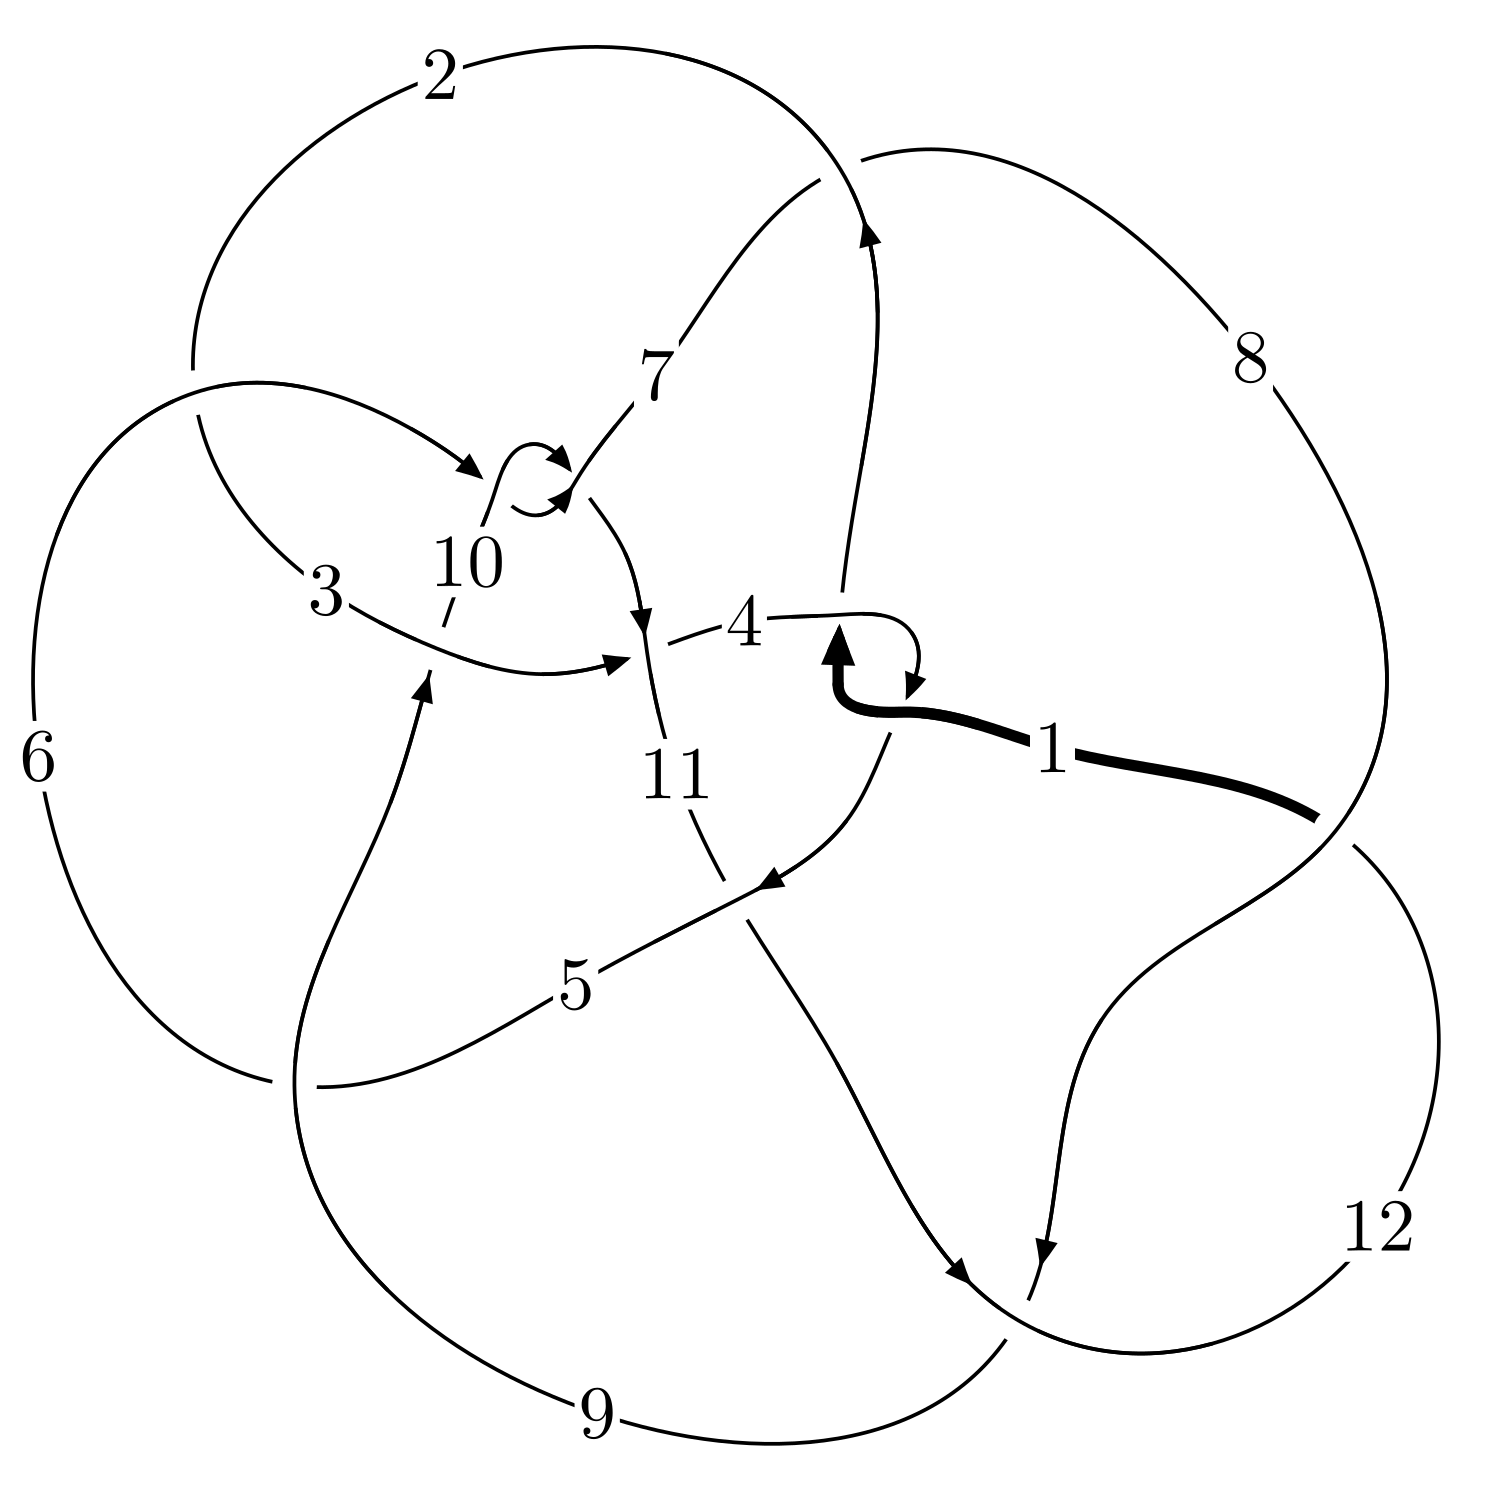
\includegraphics[width=112pt]{../../../GIT/diagram.site/Diagrams/png/1793_12a_0992.png}\\
\ \ \ A knot diagram\footnotemark}&
\allowdisplaybreaks
\textbf{Linearized knot diagam} \\
\cline{2-2}
 &
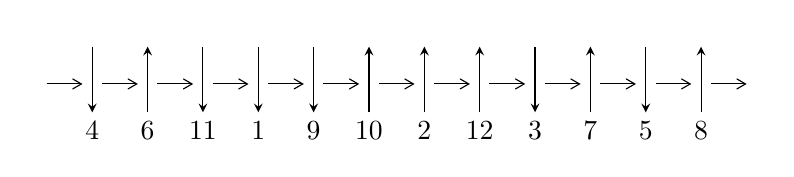
\begin{tikzpicture}[x=20pt, y=17pt]
	% nodes
	\node (C0) at (0, 0) {};
	\node (C1) at (1, 0) {};
	\node (C1U) at (1, +1) {};
	\node (C1D) at (1, -1) {4};

	\node (C2) at (2, 0) {};
	\node (C2U) at (2, +1) {};
	\node (C2D) at (2, -1) {6};

	\node (C3) at (3, 0) {};
	\node (C3U) at (3, +1) {};
	\node (C3D) at (3, -1) {11};

	\node (C4) at (4, 0) {};
	\node (C4U) at (4, +1) {};
	\node (C4D) at (4, -1) {1};

	\node (C5) at (5, 0) {};
	\node (C5U) at (5, +1) {};
	\node (C5D) at (5, -1) {9};

	\node (C6) at (6, 0) {};
	\node (C6U) at (6, +1) {};
	\node (C6D) at (6, -1) {10};

	\node (C7) at (7, 0) {};
	\node (C7U) at (7, +1) {};
	\node (C7D) at (7, -1) {2};

	\node (C8) at (8, 0) {};
	\node (C8U) at (8, +1) {};
	\node (C8D) at (8, -1) {12};

	\node (C9) at (9, 0) {};
	\node (C9U) at (9, +1) {};
	\node (C9D) at (9, -1) {3};

	\node (C10) at (10, 0) {};
	\node (C10U) at (10, +1) {};
	\node (C10D) at (10, -1) {7};

	\node (C11) at (11, 0) {};
	\node (C11U) at (11, +1) {};
	\node (C11D) at (11, -1) {5};

	\node (C12) at (12, 0) {};
	\node (C12U) at (12, +1) {};
	\node (C12D) at (12, -1) {8};
	\node (C13) at (13, 0) {};

	% arrows
	\draw[->,>={angle 60}]
	(C0) edge (C1) (C1) edge (C2) (C2) edge (C3) (C3) edge (C4) (C4) edge (C5) (C5) edge (C6) (C6) edge (C7) (C7) edge (C8) (C8) edge (C9) (C9) edge (C10) (C10) edge (C11) (C11) edge (C12) (C12) edge (C13) ;	\draw[->,>=stealth]
	(C1U) edge (C1D) (C2D) edge (C2U) (C3U) edge (C3D) (C4U) edge (C4D) (C5U) edge (C5D) (C6D) edge (C6U) (C7D) edge (C7U) (C8D) edge (C8U) (C9U) edge (C9D) (C10D) edge (C10U) (C11U) edge (C11D) (C12D) edge (C12U) ;
	\end{tikzpicture} \\
\hhline{~~} \\& 
\textbf{Solving Sequence} \\ \cline{2-2} 
 &
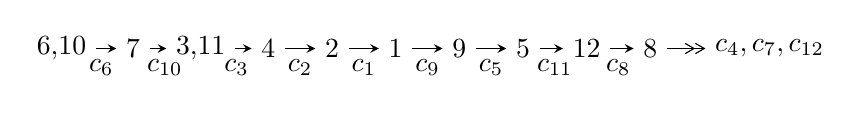
\begin{tikzpicture}[x=23pt, y=7pt]
	% node
	\node (A0) at (-1/8, 0) {6,10};
	\node (A1) at (1, 0) {7};
	\node (A2) at (33/16, 0) {3,11};
	\node (A3) at (25/8, 0) {4};
	\node (A4) at (33/8, 0) {2};
	\node (A5) at (41/8, 0) {1};
	\node (A6) at (49/8, 0) {9};
	\node (A7) at (57/8, 0) {5};
	\node (A8) at (65/8, 0) {12};
	\node (A9) at (73/8, 0) {8};
	\node (C1) at (1/2, -1) {$c_{6}$};
	\node (C2) at (3/2, -1) {$c_{10}$};
	\node (C3) at (21/8, -1) {$c_{3}$};
	\node (C4) at (29/8, -1) {$c_{2}$};
	\node (C5) at (37/8, -1) {$c_{1}$};
	\node (C6) at (45/8, -1) {$c_{9}$};
	\node (C7) at (53/8, -1) {$c_{5}$};
	\node (C8) at (61/8, -1) {$c_{11}$};
	\node (C9) at (69/8, -1) {$c_{8}$};
	\node (A10) at (11, 0) {$c_{4},c_{7},c_{12}$};

	% edge
	\draw[->,>=stealth]	
	(A0) edge (A1) (A1) edge (A2) (A2) edge (A3) (A3) edge (A4) (A4) edge (A5) (A5) edge (A6) (A6) edge (A7) (A7) edge (A8) (A8) edge (A9) ;
	\draw[->>,>={angle 60}]	
	(A9) edge (A10);
\end{tikzpicture} \\ 

\end{tabular} \\

\footnotetext{
The image of knot diagram is generated by the software ``\textbf{Draw programme}" developed by Andrew Bartholomew(\url{http://www.layer8.co.uk/maths/draw/index.htm\#Running-draw}), where we modified some parts for our purpose(\url{https://github.com/CATsTAILs/LinksPainter}).
}\phantom \\ \newline 
\centering \textbf{Ideals for irreducible components\footnotemark of $X_{\text{par}}$} 
 
\begin{align*}
I^u_{1}&=\langle 
-6.71059\times10^{901} u^{172}+5.27349\times10^{901} u^{171}+\cdots+5.37860\times10^{901} b-2.15607\times10^{903},\\
\phantom{I^u_{1}}&\phantom{= \langle  }6.55390\times10^{902} u^{172}-1.60404\times10^{903} u^{171}+\cdots+1.23708\times10^{903} a+7.01893\times10^{904},\\
\phantom{I^u_{1}}&\phantom{= \langle  }u^{173}-61 u^{171}+\cdots-1173 u+23\rangle \\
I^u_{2}&=\langle 
1.36185\times10^{44} u^{40}-3.58124\times10^{43} u^{39}+\cdots+3.88409\times10^{43} b-1.89538\times10^{45},\\
\phantom{I^u_{2}}&\phantom{= \langle  }1.79661\times10^{43} u^{40}+1.30822\times10^{43} u^{39}+\cdots+1.47328\times10^{43} a-5.14471\times10^{44},\;u^{41}- u^{40}+\cdots+29 u+11\rangle \\
\\
\end{align*}
\raggedright * 2 irreducible components of $\dim_{\mathbb{C}}=0$, with total 214 representations.\\
\footnotetext{All coefficients of polynomials are rational numbers. But the coefficients are sometimes approximated in decimal forms when there is not enough margin.}
\newpage
\renewcommand{\arraystretch}{1}
\centering \section*{I. $I^u_{1}= \langle -6.71\times10^{901} u^{172}+5.27\times10^{901} u^{171}+\cdots+5.38\times10^{901} b-2.16\times10^{903},\;6.55\times10^{902} u^{172}-1.60\times10^{903} u^{171}+\cdots+1.24\times10^{903} a+7.02\times10^{904},\;u^{173}-61 u^{171}+\cdots-1173 u+23 \rangle$}
\flushleft \textbf{(i) Arc colorings}\\
\begin{tabular}{m{7pt} m{180pt} m{7pt} m{180pt} }
\flushright $a_{6}=$&$\begin{pmatrix}1\\0\end{pmatrix}$ \\
\flushright $a_{10}=$&$\begin{pmatrix}0\\u\end{pmatrix}$ \\
\flushright $a_{7}=$&$\begin{pmatrix}1\\- u^2\end{pmatrix}$ \\
\flushright $a_{3}=$&$\begin{pmatrix}-0.529789 u^{172}+1.29664 u^{171}+\cdots+5321.00 u-56.7380\\1.24764 u^{172}-0.980457 u^{171}+\cdots-2141.18 u+40.0861\end{pmatrix}$ \\
\flushright $a_{11}=$&$\begin{pmatrix}u\\- u^3+u\end{pmatrix}$ \\
\flushright $a_{4}=$&$\begin{pmatrix}-1.65323 u^{172}+2.69220 u^{171}+\cdots+8796.48 u-123.586\\0.522388 u^{172}-0.206474 u^{171}+\cdots-328.539 u+5.33571\end{pmatrix}$ \\
\flushright $a_{2}=$&$\begin{pmatrix}-1.77743 u^{172}+2.27709 u^{171}+\cdots+7462.18 u-96.8241\\1.24764 u^{172}-0.980457 u^{171}+\cdots-2141.18 u+40.0861\end{pmatrix}$ \\
\flushright $a_{1}=$&$\begin{pmatrix}2.16146 u^{172}-3.81691 u^{171}+\cdots-6443.06 u+140.089\\2.64020 u^{172}-1.61551 u^{171}+\cdots-2165.65 u+40.4623\end{pmatrix}$ \\
\flushright $a_{9}=$&$\begin{pmatrix}-15.6581 u^{172}+13.4858 u^{171}+\cdots+28371.1 u-494.743\\-3.60652 u^{172}+2.74214 u^{171}+\cdots+3813.14 u-73.3888\end{pmatrix}$ \\
\flushright $a_{5}=$&$\begin{pmatrix}-7.26184 u^{172}+5.82108 u^{171}+\cdots+13912.4 u-229.742\\1.38948 u^{172}+0.0103074 u^{171}+\cdots+99.1447 u-3.27255\end{pmatrix}$ \\
\flushright $a_{12}=$&$\begin{pmatrix}8.70101 u^{172}-4.55347 u^{171}+\cdots-8538.66 u+129.068\\1.79058 u^{172}-1.55903 u^{171}+\cdots-2586.99 u+49.6991\end{pmatrix}$ \\
\flushright $a_{8}=$&$\begin{pmatrix}-10.6185 u^{172}+5.87960 u^{171}+\cdots+13695.9 u-228.354\\-3.31591 u^{172}+3.25383 u^{171}+\cdots+6059.20 u-117.141\end{pmatrix}$\\&\end{tabular}
\flushleft \textbf{(ii) Obstruction class $= -1$}\\~\\
\flushleft \textbf{(iii) Cusp Shapes $= -54.1766 u^{172}+34.3738 u^{171}+\cdots+59564.6 u-1133.39$}\\~\\
\newpage\renewcommand{\arraystretch}{1}
\flushleft \textbf{(iv) u-Polynomials at the component}\newline \\
\begin{tabular}{m{50pt}|m{274pt}}
Crossings & \hspace{64pt}u-Polynomials at each crossing \\
\hline $$\begin{aligned}c_{1},c_{4}\end{aligned}$$&$\begin{aligned}
&u^{173}+10 u^{172}+\cdots-19296 u+2479
\end{aligned}$\\
\hline $$\begin{aligned}c_{2}\end{aligned}$$&$\begin{aligned}
&u^{173}-11 u^{172}+\cdots+81 u+1
\end{aligned}$\\
\hline $$\begin{aligned}c_{3}\end{aligned}$$&$\begin{aligned}
&u^{173}+5 u^{171}+\cdots-63604 u+4777
\end{aligned}$\\
\hline $$\begin{aligned}c_{5}\end{aligned}$$&$\begin{aligned}
&u^{173}+5 u^{172}+\cdots-146967068577 u-20660319509
\end{aligned}$\\
\hline $$\begin{aligned}c_{6},c_{10}\end{aligned}$$&$\begin{aligned}
&u^{173}-61 u^{171}+\cdots-1173 u-23
\end{aligned}$\\
\hline $$\begin{aligned}c_{7}\end{aligned}$$&$\begin{aligned}
&u^{173}+u^{172}+\cdots+118309218 u-11032501
\end{aligned}$\\
\hline $$\begin{aligned}c_{8},c_{12}\end{aligned}$$&$\begin{aligned}
&u^{173}-5 u^{172}+\cdots+16696 u+15296
\end{aligned}$\\
\hline $$\begin{aligned}c_{9}\end{aligned}$$&$\begin{aligned}
&u^{173}+u^{172}+\cdots-14 u+4
\end{aligned}$\\
\hline $$\begin{aligned}c_{11}\end{aligned}$$&$\begin{aligned}
&u^{173}-21 u^{171}+\cdots-2568295 u+328021
\end{aligned}$\\
\hline
\end{tabular}\\~\\
\newpage\renewcommand{\arraystretch}{1}
\flushleft \textbf{(v) Riley Polynomials at the component}\newline \\
\begin{tabular}{m{50pt}|m{274pt}}
Crossings & \hspace{64pt}Riley Polynomials at each crossing \\
\hline $$\begin{aligned}c_{1},c_{4}\end{aligned}$$&$\begin{aligned}
&y^{173}+110 y^{172}+\cdots-487431164 y-6145441
\end{aligned}$\\
\hline $$\begin{aligned}c_{2}\end{aligned}$$&$\begin{aligned}
&y^{173}+15 y^{172}+\cdots+6111 y-1
\end{aligned}$\\
\hline $$\begin{aligned}c_{3}\end{aligned}$$&$\begin{aligned}
&y^{173}+10 y^{172}+\cdots-4426368712 y-22819729
\end{aligned}$\\
\hline $$\begin{aligned}c_{5}\end{aligned}$$&$\begin{aligned}
&y^{173}-101 y^{172}+\cdots+2.92\times10^{22} y-4.27\times10^{20}
\end{aligned}$\\
\hline $$\begin{aligned}c_{6},c_{10}\end{aligned}$$&$\begin{aligned}
&y^{173}-122 y^{172}+\cdots+882901 y-529
\end{aligned}$\\
\hline $$\begin{aligned}c_{7}\end{aligned}$$&$\begin{aligned}
&y^{173}+43 y^{172}+\cdots+128804976616151910 y-121716078315001
\end{aligned}$\\
\hline $$\begin{aligned}c_{8},c_{12}\end{aligned}$$&$\begin{aligned}
&y^{173}+105 y^{172}+\cdots-8693357120 y-233967616
\end{aligned}$\\
\hline $$\begin{aligned}c_{9}\end{aligned}$$&$\begin{aligned}
&y^{173}- y^{172}+\cdots-964 y-16
\end{aligned}$\\
\hline $$\begin{aligned}c_{11}\end{aligned}$$&$\begin{aligned}
&y^{173}-42 y^{172}+\cdots-3575854983007 y-107597776441
\end{aligned}$\\
\hline
\end{tabular}\\~\\
\newpage\flushleft \textbf{(vi) Complex Volumes and Cusp Shapes}
$$\begin{array}{c|c|c}  
\text{Solutions to }I^u_{1}& \I (\text{vol} + \sqrt{-1}CS) & \text{Cusp shape}\\
 \hline 
\begin{aligned}
u &= \phantom{-}0.969243 + 0.220547 I \\
a &= -1.052810 + 0.930178 I \\
b &= \phantom{-}1.25731 + 0.70948 I\end{aligned}
 & \phantom{-}1.62467 + 4.25995 I & \phantom{-0.000000 } 0 \\ \hline\begin{aligned}
u &= \phantom{-}0.969243 - 0.220547 I \\
a &= -1.052810 - 0.930178 I \\
b &= \phantom{-}1.25731 - 0.70948 I\end{aligned}
 & \phantom{-}1.62467 - 4.25995 I & \phantom{-0.000000 } 0 \\ \hline\begin{aligned}
u &= -0.967361 + 0.222779 I \\
a &= \phantom{-}0.185385 + 0.167139 I \\
b &= \phantom{-}1.44819 + 2.43454 I\end{aligned}
 & -1.56945 - 10.43610 I & \phantom{-0.000000 } 0 \\ \hline\begin{aligned}
u &= -0.967361 - 0.222779 I \\
a &= \phantom{-}0.185385 - 0.167139 I \\
b &= \phantom{-}1.44819 - 2.43454 I\end{aligned}
 & -1.56945 + 10.43610 I & \phantom{-0.000000 } 0 \\ \hline\begin{aligned}
u &= -0.122560 + 1.003480 I \\
a &= -0.724326 - 1.006380 I \\
b &= -0.313088 - 0.910696 I\end{aligned}
 & -5.96418 - 1.53799 I & \phantom{-0.000000 } 0 \\ \hline\begin{aligned}
u &= -0.122560 - 1.003480 I \\
a &= -0.724326 + 1.006380 I \\
b &= -0.313088 + 0.910696 I\end{aligned}
 & -5.96418 + 1.53799 I & \phantom{-0.000000 } 0 \\ \hline\begin{aligned}
u &= \phantom{-}0.951040 + 0.268610 I \\
a &= -0.478403 + 1.023580 I \\
b &= \phantom{-}0.28013 + 1.77652 I\end{aligned}
 & -0.68234 + 5.89789 I & \phantom{-0.000000 } 0 \\ \hline\begin{aligned}
u &= \phantom{-}0.951040 - 0.268610 I \\
a &= -0.478403 - 1.023580 I \\
b &= \phantom{-}0.28013 - 1.77652 I\end{aligned}
 & -0.68234 - 5.89789 I & \phantom{-0.000000 } 0 \\ \hline\begin{aligned}
u &= -1.009900 + 0.132134 I \\
a &= \phantom{-}0.358996 - 1.240550 I \\
b &= -0.60699 - 1.28490 I\end{aligned}
 & \phantom{-}3.59664 - 2.11116 I & \phantom{-0.000000 } 0 \\ \hline\begin{aligned}
u &= -1.009900 - 0.132134 I \\
a &= \phantom{-}0.358996 + 1.240550 I \\
b &= -0.60699 + 1.28490 I\end{aligned}
 & \phantom{-}3.59664 + 2.11116 I & \phantom{-0.000000 } 0\\
 \hline 
 \end{array}$$\newpage$$\begin{array}{c|c|c}  
\text{Solutions to }I^u_{1}& \I (\text{vol} + \sqrt{-1}CS) & \text{Cusp shape}\\
 \hline 
\begin{aligned}
u &= -0.941710 + 0.259548 I \\
a &= \phantom{-}2.23225 - 0.37220 I \\
b &= -0.136987 + 0.157446 I\end{aligned}
 & \phantom{-}2.11551 - 5.14420 I & \phantom{-0.000000 } 0 \\ \hline\begin{aligned}
u &= -0.941710 - 0.259548 I \\
a &= \phantom{-}2.23225 + 0.37220 I \\
b &= -0.136987 - 0.157446 I\end{aligned}
 & \phantom{-}2.11551 + 5.14420 I & \phantom{-0.000000 } 0 \\ \hline\begin{aligned}
u &= \phantom{-}1.020070 + 0.082123 I \\
a &= \phantom{-}1.031600 + 0.780816 I \\
b &= -1.48063 + 0.73015 I\end{aligned}
 & \phantom{-}0.31938 - 3.49441 I & \phantom{-0.000000 } 0 \\ \hline\begin{aligned}
u &= \phantom{-}1.020070 - 0.082123 I \\
a &= \phantom{-}1.031600 - 0.780816 I \\
b &= -1.48063 - 0.73015 I\end{aligned}
 & \phantom{-}0.31938 + 3.49441 I & \phantom{-0.000000 } 0 \\ \hline\begin{aligned}
u &= -1.001830 + 0.233287 I \\
a &= -1.61373 - 0.43084 I \\
b &= \phantom{-}1.019820 - 0.686855 I\end{aligned}
 & -0.02377 - 5.78752 I & \phantom{-0.000000 } 0 \\ \hline\begin{aligned}
u &= -1.001830 - 0.233287 I \\
a &= -1.61373 + 0.43084 I \\
b &= \phantom{-}1.019820 + 0.686855 I\end{aligned}
 & -0.02377 + 5.78752 I & \phantom{-0.000000 } 0 \\ \hline\begin{aligned}
u &= \phantom{-}0.136236 + 1.025890 I \\
a &= -0.719633 + 0.799077 I \\
b &= -0.650525 + 0.788882 I\end{aligned}
 & -3.46252 - 4.21752 I & \phantom{-0.000000 } 0 \\ \hline\begin{aligned}
u &= \phantom{-}0.136236 - 1.025890 I \\
a &= -0.719633 - 0.799077 I \\
b &= -0.650525 - 0.788882 I\end{aligned}
 & -3.46252 + 4.21752 I & \phantom{-0.000000 } 0 \\ \hline\begin{aligned}
u &= -0.167977 + 0.950127 I \\
a &= -0.290002 + 1.037440 I \\
b &= -0.951466 + 0.745473 I\end{aligned}
 & -3.68721 - 3.27523 I & \phantom{-0.000000 } 0 \\ \hline\begin{aligned}
u &= -0.167977 - 0.950127 I \\
a &= -0.290002 - 1.037440 I \\
b &= -0.951466 - 0.745473 I\end{aligned}
 & -3.68721 + 3.27523 I & \phantom{-0.000000 } 0\\
 \hline 
 \end{array}$$\newpage$$\begin{array}{c|c|c}  
\text{Solutions to }I^u_{1}& \I (\text{vol} + \sqrt{-1}CS) & \text{Cusp shape}\\
 \hline 
\begin{aligned}
u &= -0.910982 + 0.299524 I \\
a &= \phantom{-}0.34574 + 2.05281 I \\
b &= -0.302013 + 0.801161 I\end{aligned}
 & -0.46105 - 2.18860 I & \phantom{-0.000000 } 0 \\ \hline\begin{aligned}
u &= -0.910982 - 0.299524 I \\
a &= \phantom{-}0.34574 - 2.05281 I \\
b &= -0.302013 - 0.801161 I\end{aligned}
 & -0.46105 + 2.18860 I & \phantom{-0.000000 } 0 \\ \hline\begin{aligned}
u &= -0.005164 + 1.041260 I \\
a &= \phantom{-}0.639436 + 0.862373 I \\
b &= \phantom{-}0.360312 + 1.070660 I\end{aligned}
 & -6.97562 + 2.24381 I & \phantom{-0.000000 } 0 \\ \hline\begin{aligned}
u &= -0.005164 - 1.041260 I \\
a &= \phantom{-}0.639436 - 0.862373 I \\
b &= \phantom{-}0.360312 - 1.070660 I\end{aligned}
 & -6.97562 - 2.24381 I & \phantom{-0.000000 } 0 \\ \hline\begin{aligned}
u &= \phantom{-}1.023210 + 0.250565 I \\
a &= \phantom{-}2.07776 + 0.94856 I \\
b &= -0.203059 - 0.266347 I\end{aligned}
 & -1.13240 + 11.02240 I & \phantom{-0.000000 } 0 \\ \hline\begin{aligned}
u &= \phantom{-}1.023210 - 0.250565 I \\
a &= \phantom{-}2.07776 - 0.94856 I \\
b &= -0.203059 + 0.266347 I\end{aligned}
 & -1.13240 - 11.02240 I & \phantom{-0.000000 } 0 \\ \hline\begin{aligned}
u &= -0.179225 + 1.040520 I \\
a &= -0.898061 - 0.760638 I \\
b &= -0.768989 - 0.984083 I\end{aligned}
 & -7.85520 + 8.35950 I & \phantom{-0.000000 } 0 \\ \hline\begin{aligned}
u &= -0.179225 - 1.040520 I \\
a &= -0.898061 + 0.760638 I \\
b &= -0.768989 + 0.984083 I\end{aligned}
 & -7.85520 - 8.35950 I & \phantom{-0.000000 } 0 \\ \hline\begin{aligned}
u &= \phantom{-}0.901239 + 0.244418 I \\
a &= -0.800546 + 0.899555 I \\
b &= \phantom{-}1.33330 + 0.76864 I\end{aligned}
 & \phantom{-}1.61175 + 4.35594 I & \phantom{-0.000000 } 0 \\ \hline\begin{aligned}
u &= \phantom{-}0.901239 - 0.244418 I \\
a &= -0.800546 - 0.899555 I \\
b &= \phantom{-}1.33330 - 0.76864 I\end{aligned}
 & \phantom{-}1.61175 - 4.35594 I & \phantom{-0.000000 } 0\\
 \hline 
 \end{array}$$\newpage$$\begin{array}{c|c|c}  
\text{Solutions to }I^u_{1}& \I (\text{vol} + \sqrt{-1}CS) & \text{Cusp shape}\\
 \hline 
\begin{aligned}
u &= -0.886423 + 0.608296 I \\
a &= -0.417111 - 0.851974 I \\
b &= \phantom{-}1.51474 - 0.98438 I\end{aligned}
 & -3.01484 - 6.95211 I & \phantom{-0.000000 } 0 \\ \hline\begin{aligned}
u &= -0.886423 - 0.608296 I \\
a &= -0.417111 + 0.851974 I \\
b &= \phantom{-}1.51474 + 0.98438 I\end{aligned}
 & -3.01484 + 6.95211 I & \phantom{-0.000000 } 0 \\ \hline\begin{aligned}
u &= -1.073010 + 0.129958 I \\
a &= -0.776007 + 0.912568 I \\
b &= \phantom{-}0.833781 + 0.132686 I\end{aligned}
 & \phantom{-}2.52711 - 0.99224 I & \phantom{-0.000000 } 0 \\ \hline\begin{aligned}
u &= -1.073010 - 0.129958 I \\
a &= -0.776007 - 0.912568 I \\
b &= \phantom{-}0.833781 - 0.132686 I\end{aligned}
 & \phantom{-}2.52711 + 0.99224 I & \phantom{-0.000000 } 0 \\ \hline\begin{aligned}
u &= -0.903819 + 0.600056 I \\
a &= -0.194228 + 0.097503 I \\
b &= -0.697492 - 1.036150 I\end{aligned}
 & -1.60144 - 1.97820 I & \phantom{-0.000000 } 0 \\ \hline\begin{aligned}
u &= -0.903819 - 0.600056 I \\
a &= -0.194228 - 0.097503 I \\
b &= -0.697492 + 1.036150 I\end{aligned}
 & -1.60144 + 1.97820 I & \phantom{-0.000000 } 0 \\ \hline\begin{aligned}
u &= \phantom{-}0.722477 + 0.814466 I \\
a &= \phantom{-}0.740815 + 0.042360 I \\
b &= \phantom{-}0.734908 - 0.521689 I\end{aligned}
 & \phantom{-}0.530642 - 0.857914 I & \phantom{-0.000000 } 0 \\ \hline\begin{aligned}
u &= \phantom{-}0.722477 - 0.814466 I \\
a &= \phantom{-}0.740815 - 0.042360 I \\
b &= \phantom{-}0.734908 + 0.521689 I\end{aligned}
 & \phantom{-}0.530642 + 0.857914 I & \phantom{-0.000000 } 0 \\ \hline\begin{aligned}
u &= \phantom{-}0.878159 + 0.242664 I \\
a &= -0.098780 + 0.283426 I \\
b &= -0.554255 + 1.293440 I\end{aligned}
 & -0.73676 + 2.10314 I & \phantom{-0.000000 } 0 \\ \hline\begin{aligned}
u &= \phantom{-}0.878159 - 0.242664 I \\
a &= -0.098780 - 0.283426 I \\
b &= -0.554255 - 1.293440 I\end{aligned}
 & -0.73676 - 2.10314 I & \phantom{-0.000000 } 0\\
 \hline 
 \end{array}$$\newpage$$\begin{array}{c|c|c}  
\text{Solutions to }I^u_{1}& \I (\text{vol} + \sqrt{-1}CS) & \text{Cusp shape}\\
 \hline 
\begin{aligned}
u &= -0.910249 + 0.037015 I \\
a &= -0.47849 - 1.45705 I \\
b &= \phantom{-}0.753338 - 0.765683 I\end{aligned}
 & \phantom{-}1.40037 - 0.58570 I & \phantom{-0.000000 } 0 \\ \hline\begin{aligned}
u &= -0.910249 - 0.037015 I \\
a &= -0.47849 + 1.45705 I \\
b &= \phantom{-}0.753338 + 0.765683 I\end{aligned}
 & \phantom{-}1.40037 + 0.58570 I & \phantom{-0.000000 } 0 \\ \hline\begin{aligned}
u &= \phantom{-}1.079010 + 0.206227 I \\
a &= -0.123987 - 0.360311 I \\
b &= \phantom{-}1.47315 - 0.91538 I\end{aligned}
 & \phantom{-}4.03967 + 5.41750 I & \phantom{-0.000000 } 0 \\ \hline\begin{aligned}
u &= \phantom{-}1.079010 - 0.206227 I \\
a &= -0.123987 + 0.360311 I \\
b &= \phantom{-}1.47315 + 0.91538 I\end{aligned}
 & \phantom{-}4.03967 - 5.41750 I & \phantom{-0.000000 } 0 \\ \hline\begin{aligned}
u &= \phantom{-}1.008880 + 0.455136 I \\
a &= \phantom{-}1.146700 + 0.496191 I \\
b &= \phantom{-}0.108682 - 0.153213 I\end{aligned}
 & -3.02207 + 0.95034 I & \phantom{-0.000000 } 0 \\ \hline\begin{aligned}
u &= \phantom{-}1.008880 - 0.455136 I \\
a &= \phantom{-}1.146700 - 0.496191 I \\
b &= \phantom{-}0.108682 + 0.153213 I\end{aligned}
 & -3.02207 - 0.95034 I & \phantom{-0.000000 } 0 \\ \hline\begin{aligned}
u &= -0.858386 + 0.230562 I \\
a &= \phantom{-}1.091710 + 0.363015 I \\
b &= -1.81940 + 0.94635 I\end{aligned}
 & -5.46005 + 1.54949 I & \phantom{-0.000000 } 0 \\ \hline\begin{aligned}
u &= -0.858386 - 0.230562 I \\
a &= \phantom{-}1.091710 - 0.363015 I \\
b &= -1.81940 - 0.94635 I\end{aligned}
 & -5.46005 - 1.54949 I & \phantom{-0.000000 } 0 \\ \hline\begin{aligned}
u &= \phantom{-}0.685350 + 0.557198 I \\
a &= \phantom{-}0.192676 - 0.505351 I \\
b &= -0.838605 + 0.312875 I\end{aligned}
 & -1.88020 + 2.17309 I & \phantom{-0.000000 } 0 \\ \hline\begin{aligned}
u &= \phantom{-}0.685350 - 0.557198 I \\
a &= \phantom{-}0.192676 + 0.505351 I \\
b &= -0.838605 - 0.312875 I\end{aligned}
 & -1.88020 - 2.17309 I & \phantom{-0.000000 } 0\\
 \hline 
 \end{array}$$\newpage$$\begin{array}{c|c|c}  
\text{Solutions to }I^u_{1}& \I (\text{vol} + \sqrt{-1}CS) & \text{Cusp shape}\\
 \hline 
\begin{aligned}
u &= \phantom{-}0.419039 + 0.770002 I \\
a &= -1.171560 + 0.741643 I \\
b &= -0.508847 + 0.460575 I\end{aligned}
 & -4.21165 - 3.97894 I & \phantom{-0.000000 } 0 \\ \hline\begin{aligned}
u &= \phantom{-}0.419039 - 0.770002 I \\
a &= -1.171560 - 0.741643 I \\
b &= -0.508847 - 0.460575 I\end{aligned}
 & -4.21165 + 3.97894 I & \phantom{-0.000000 } 0 \\ \hline\begin{aligned}
u &= \phantom{-}0.757319 + 0.438938 I \\
a &= -0.16686 - 1.98211 I \\
b &= -0.502869 - 0.956805 I\end{aligned}
 & -3.29399 + 8.42223 I & \phantom{-0.000000 } 0 \\ \hline\begin{aligned}
u &= \phantom{-}0.757319 - 0.438938 I \\
a &= -0.16686 + 1.98211 I \\
b &= -0.502869 + 0.956805 I\end{aligned}
 & -3.29399 - 8.42223 I & \phantom{-0.000000 } 0 \\ \hline\begin{aligned}
u &= \phantom{-}0.182868 + 1.127140 I \\
a &= -0.099297 - 0.868525 I \\
b &= -0.698346 - 1.089340 I\end{aligned}
 & -4.82462 + 3.35490 I & \phantom{-0.000000 } 0 \\ \hline\begin{aligned}
u &= \phantom{-}0.182868 - 1.127140 I \\
a &= -0.099297 + 0.868525 I \\
b &= -0.698346 + 1.089340 I\end{aligned}
 & -4.82462 - 3.35490 I & \phantom{-0.000000 } 0 \\ \hline\begin{aligned}
u &= \phantom{-}0.810558 + 0.253566 I \\
a &= -2.39009 - 0.15928 I \\
b &= \phantom{-}0.007354 + 0.444463 I\end{aligned}
 & -5.77653 + 4.38873 I & \phantom{-0.000000 } 0 \\ \hline\begin{aligned}
u &= \phantom{-}0.810558 - 0.253566 I \\
a &= -2.39009 + 0.15928 I \\
b &= \phantom{-}0.007354 - 0.444463 I\end{aligned}
 & -5.77653 - 4.38873 I & \phantom{-0.000000 } 0 \\ \hline\begin{aligned}
u &= -0.032255 + 1.171010 I \\
a &= \phantom{-}0.677224 + 0.810296 I \\
b &= \phantom{-}0.777621 + 1.012520 I\end{aligned}
 & -4.8125 + 14.7446 I & \phantom{-0.000000 } 0 \\ \hline\begin{aligned}
u &= -0.032255 - 1.171010 I \\
a &= \phantom{-}0.677224 - 0.810296 I \\
b &= \phantom{-}0.777621 - 1.012520 I\end{aligned}
 & -4.8125 - 14.7446 I & \phantom{-0.000000 } 0\\
 \hline 
 \end{array}$$\newpage$$\begin{array}{c|c|c}  
\text{Solutions to }I^u_{1}& \I (\text{vol} + \sqrt{-1}CS) & \text{Cusp shape}\\
 \hline 
\begin{aligned}
u &= \phantom{-}0.004153 + 1.173180 I \\
a &= \phantom{-}0.621616 - 0.800224 I \\
b &= \phantom{-}0.628100 - 0.923295 I\end{aligned}
 & -0.86051 - 8.28933 I & \phantom{-0.000000 } 0 \\ \hline\begin{aligned}
u &= \phantom{-}0.004153 - 1.173180 I \\
a &= \phantom{-}0.621616 + 0.800224 I \\
b &= \phantom{-}0.628100 + 0.923295 I\end{aligned}
 & -0.86051 + 8.28933 I & \phantom{-0.000000 } 0 \\ \hline\begin{aligned}
u &= -1.160770 + 0.172269 I \\
a &= \phantom{-}0.251287 + 0.297848 I \\
b &= -0.620853 + 0.121311 I\end{aligned}
 & \phantom{-}1.95157 - 0.09545 I & \phantom{-0.000000 } 0 \\ \hline\begin{aligned}
u &= -1.160770 - 0.172269 I \\
a &= \phantom{-}0.251287 - 0.297848 I \\
b &= -0.620853 - 0.121311 I\end{aligned}
 & \phantom{-}1.95157 + 0.09545 I & \phantom{-0.000000 } 0 \\ \hline\begin{aligned}
u &= -1.102500 + 0.403399 I \\
a &= -0.64337 - 1.36102 I \\
b &= \phantom{-}1.25118 - 1.39287 I\end{aligned}
 & \phantom{-}2.20201 - 6.60941 I & \phantom{-0.000000 } 0 \\ \hline\begin{aligned}
u &= -1.102500 - 0.403399 I \\
a &= -0.64337 + 1.36102 I \\
b &= \phantom{-}1.25118 + 1.39287 I\end{aligned}
 & \phantom{-}2.20201 + 6.60941 I & \phantom{-0.000000 } 0 \\ \hline\begin{aligned}
u &= \phantom{-}0.783807 + 0.204550 I \\
a &= \phantom{-}0.43137 - 2.27060 I \\
b &= -0.062834 - 1.100940 I\end{aligned}
 & -5.93852 - 1.91924 I & \phantom{-0.000000 } 0 \\ \hline\begin{aligned}
u &= \phantom{-}0.783807 - 0.204550 I \\
a &= \phantom{-}0.43137 + 2.27060 I \\
b &= -0.062834 + 1.100940 I\end{aligned}
 & -5.93852 + 1.91924 I & \phantom{-0.000000 } 0 \\ \hline\begin{aligned}
u &= -0.786568 + 0.168902 I \\
a &= -0.404782 - 0.074901 I \\
b &= -0.69002 - 2.25440 I\end{aligned}
 & -5.77655 - 3.77297 I & \phantom{-0.000000 } 0 \\ \hline\begin{aligned}
u &= -0.786568 - 0.168902 I \\
a &= -0.404782 + 0.074901 I \\
b &= -0.69002 + 2.25440 I\end{aligned}
 & -5.77655 + 3.77297 I & \phantom{-0.000000 } 0\\
 \hline 
 \end{array}$$\newpage$$\begin{array}{c|c|c}  
\text{Solutions to }I^u_{1}& \I (\text{vol} + \sqrt{-1}CS) & \text{Cusp shape}\\
 \hline 
\begin{aligned}
u &= -0.096945 + 1.208110 I \\
a &= \phantom{-}0.285525 + 0.606083 I \\
b &= \phantom{-}0.496297 + 1.208820 I\end{aligned}
 & -5.85740 + 0.93686 I & \phantom{-0.000000 } 0 \\ \hline\begin{aligned}
u &= -0.096945 - 1.208110 I \\
a &= \phantom{-}0.285525 - 0.606083 I \\
b &= \phantom{-}0.496297 - 1.208820 I\end{aligned}
 & -5.85740 - 0.93686 I & \phantom{-0.000000 } 0 \\ \hline\begin{aligned}
u &= \phantom{-}0.766704 + 0.109869 I \\
a &= -0.073871 + 0.880786 I \\
b &= -1.038940 - 0.028975 I\end{aligned}
 & -0.32041 + 4.36664 I & \phantom{-0.000000 } 0 \\ \hline\begin{aligned}
u &= \phantom{-}0.766704 - 0.109869 I \\
a &= -0.073871 - 0.880786 I \\
b &= -1.038940 + 0.028975 I\end{aligned}
 & -0.32041 - 4.36664 I & \phantom{-0.000000 } 0 \\ \hline\begin{aligned}
u &= \phantom{-}1.200650 + 0.271618 I \\
a &= -0.265384 + 0.267536 I \\
b &= \phantom{-}1.58241 + 0.43184 I\end{aligned}
 & \phantom{-}3.49282 + 6.04510 I & \phantom{-0.000000 } 0 \\ \hline\begin{aligned}
u &= \phantom{-}1.200650 - 0.271618 I \\
a &= -0.265384 - 0.267536 I \\
b &= \phantom{-}1.58241 - 0.43184 I\end{aligned}
 & \phantom{-}3.49282 - 6.04510 I & \phantom{-0.000000 } 0 \\ \hline\begin{aligned}
u &= -0.368818 + 0.672839 I \\
a &= \phantom{-}0.818687 - 0.095745 I \\
b &= \phantom{-}0.500821 - 0.511438 I\end{aligned}
 & -0.78139 - 3.14198 I & \phantom{-0.000000 } 0 \\ \hline\begin{aligned}
u &= -0.368818 - 0.672839 I \\
a &= \phantom{-}0.818687 + 0.095745 I \\
b &= \phantom{-}0.500821 + 0.511438 I\end{aligned}
 & -0.78139 + 3.14198 I & \phantom{-0.000000 } 0 \\ \hline\begin{aligned}
u &= -1.219470 + 0.205127 I \\
a &= -1.03405 - 1.35713 I \\
b &= \phantom{-}0.740843 - 0.645709 I\end{aligned}
 & \phantom{-}5.58472 - 5.07772 I & \phantom{-0.000000 } 0 \\ \hline\begin{aligned}
u &= -1.219470 - 0.205127 I \\
a &= -1.03405 + 1.35713 I \\
b &= \phantom{-}0.740843 + 0.645709 I\end{aligned}
 & \phantom{-}5.58472 + 5.07772 I & \phantom{-0.000000 } 0\\
 \hline 
 \end{array}$$\newpage$$\begin{array}{c|c|c}  
\text{Solutions to }I^u_{1}& \I (\text{vol} + \sqrt{-1}CS) & \text{Cusp shape}\\
 \hline 
\begin{aligned}
u &= \phantom{-}1.156010 + 0.445248 I \\
a &= -0.417710 + 1.287460 I \\
b &= \phantom{-}1.37006 + 0.97818 I\end{aligned}
 & \phantom{-}2.85416 + 5.29441 I & \phantom{-0.000000 } 0 \\ \hline\begin{aligned}
u &= \phantom{-}1.156010 - 0.445248 I \\
a &= -0.417710 - 1.287460 I \\
b &= \phantom{-}1.37006 - 0.97818 I\end{aligned}
 & \phantom{-}2.85416 - 5.29441 I & \phantom{-0.000000 } 0 \\ \hline\begin{aligned}
u &= \phantom{-}0.759259\phantom{ +0.000000I} \\
a &= \phantom{-}1.21796\phantom{ +0.000000I} \\
b &= -1.58398\phantom{ +0.000000I}\end{aligned}
 & -1.67990\phantom{ +0.000000I} & \phantom{-0.000000 } 0 \\ \hline\begin{aligned}
u &= -0.749218\phantom{ +0.000000I} \\
a &= -2.97064\phantom{ +0.000000I} \\
b &= -0.0127734\phantom{ +0.000000I}\end{aligned}
 & -1.63607\phantom{ +0.000000I} & \phantom{-0.000000 } 0 \\ \hline\begin{aligned}
u &= -1.121570 + 0.562084 I \\
a &= \phantom{-}0.163020 - 0.973628 I \\
b &= \phantom{-}1.110900 - 0.390923 I\end{aligned}
 & \phantom{-}2.26211 - 2.51652 I & \phantom{-0.000000 } 0 \\ \hline\begin{aligned}
u &= -1.121570 - 0.562084 I \\
a &= \phantom{-}0.163020 + 0.973628 I \\
b &= \phantom{-}1.110900 + 0.390923 I\end{aligned}
 & \phantom{-}2.26211 + 2.51652 I & \phantom{-0.000000 } 0 \\ \hline\begin{aligned}
u &= -1.252570 + 0.183974 I \\
a &= \phantom{-}0.296046 + 0.701703 I \\
b &= -1.43761 + 1.92411 I\end{aligned}
 & \phantom{-}1.81439 - 9.64166 I & \phantom{-0.000000 } 0 \\ \hline\begin{aligned}
u &= -1.252570 - 0.183974 I \\
a &= \phantom{-}0.296046 - 0.701703 I \\
b &= -1.43761 - 1.92411 I\end{aligned}
 & \phantom{-}1.81439 + 9.64166 I & \phantom{-0.000000 } 0 \\ \hline\begin{aligned}
u &= \phantom{-}0.410556 + 1.198760 I \\
a &= -0.540811 - 0.091650 I \\
b &= -0.737529 + 0.107259 I\end{aligned}
 & \phantom{-}0.87054 - 6.12136 I & \phantom{-0.000000 } 0 \\ \hline\begin{aligned}
u &= \phantom{-}0.410556 - 1.198760 I \\
a &= -0.540811 + 0.091650 I \\
b &= -0.737529 - 0.107259 I\end{aligned}
 & \phantom{-}0.87054 + 6.12136 I & \phantom{-0.000000 } 0\\
 \hline 
 \end{array}$$\newpage$$\begin{array}{c|c|c}  
\text{Solutions to }I^u_{1}& \I (\text{vol} + \sqrt{-1}CS) & \text{Cusp shape}\\
 \hline 
\begin{aligned}
u &= \phantom{-}1.157080 + 0.533898 I \\
a &= -0.212976 + 0.382913 I \\
b &= \phantom{-}0.085770 + 1.017750 I\end{aligned}
 & -1.90982 + 2.48807 I & \phantom{-0.000000 } 0 \\ \hline\begin{aligned}
u &= \phantom{-}1.157080 - 0.533898 I \\
a &= -0.212976 - 0.382913 I \\
b &= \phantom{-}0.085770 - 1.017750 I\end{aligned}
 & -1.90982 - 2.48807 I & \phantom{-0.000000 } 0 \\ \hline\begin{aligned}
u &= -0.725390 + 1.058350 I \\
a &= -0.220840 + 0.450227 I \\
b &= -0.526215 + 0.205867 I\end{aligned}
 & \phantom{-}3.14897 + 0.40252 I & \phantom{-0.000000 } 0 \\ \hline\begin{aligned}
u &= -0.725390 - 1.058350 I \\
a &= -0.220840 - 0.450227 I \\
b &= -0.526215 - 0.205867 I\end{aligned}
 & \phantom{-}3.14897 - 0.40252 I & \phantom{-0.000000 } 0 \\ \hline\begin{aligned}
u &= \phantom{-}1.191820 + 0.489960 I \\
a &= -0.316041 + 1.049930 I \\
b &= \phantom{-}1.22005 + 0.87336 I\end{aligned}
 & \phantom{-}2.71899 + 5.49712 I & \phantom{-0.000000 } 0 \\ \hline\begin{aligned}
u &= \phantom{-}1.191820 - 0.489960 I \\
a &= -0.316041 - 1.049930 I \\
b &= \phantom{-}1.22005 - 0.87336 I\end{aligned}
 & \phantom{-}2.71899 - 5.49712 I & \phantom{-0.000000 } 0 \\ \hline\begin{aligned}
u &= \phantom{-}1.288050 + 0.181306 I \\
a &= \phantom{-}0.157721 - 1.163590 I \\
b &= -0.0435054 - 0.1013280 I\end{aligned}
 & \phantom{-}4.89026 + 3.20957 I & \phantom{-0.000000 } 0 \\ \hline\begin{aligned}
u &= \phantom{-}1.288050 - 0.181306 I \\
a &= \phantom{-}0.157721 + 1.163590 I \\
b &= -0.0435054 + 0.1013280 I\end{aligned}
 & \phantom{-}4.89026 - 3.20957 I & \phantom{-0.000000 } 0 \\ \hline\begin{aligned}
u &= -0.682522 + 0.131631 I \\
a &= \phantom{-}0.94611 - 1.22570 I \\
b &= -0.550588 + 0.135442 I\end{aligned}
 & \phantom{-}2.74796 + 0.70076 I & \phantom{-0.000000 } 0 \\ \hline\begin{aligned}
u &= -0.682522 - 0.131631 I \\
a &= \phantom{-}0.94611 + 1.22570 I \\
b &= -0.550588 - 0.135442 I\end{aligned}
 & \phantom{-}2.74796 - 0.70076 I & \phantom{-0.000000 } 0\\
 \hline 
 \end{array}$$\newpage$$\begin{array}{c|c|c}  
\text{Solutions to }I^u_{1}& \I (\text{vol} + \sqrt{-1}CS) & \text{Cusp shape}\\
 \hline 
\begin{aligned}
u &= -1.227500 + 0.539315 I \\
a &= -0.415190 - 0.786644 I \\
b &= \phantom{-}1.33725 - 1.23938 I\end{aligned}
 & -2.61566 - 7.02854 I & \phantom{-0.000000 } 0 \\ \hline\begin{aligned}
u &= -1.227500 - 0.539315 I \\
a &= -0.415190 + 0.786644 I \\
b &= \phantom{-}1.33725 + 1.23938 I\end{aligned}
 & -2.61566 + 7.02854 I & \phantom{-0.000000 } 0 \\ \hline\begin{aligned}
u &= -1.329220 + 0.228470 I \\
a &= \phantom{-}0.370944 + 1.084410 I \\
b &= -0.487068 + 0.157170 I\end{aligned}
 & \phantom{-}4.16915 - 4.28201 I & \phantom{-0.000000 } 0 \\ \hline\begin{aligned}
u &= -1.329220 - 0.228470 I \\
a &= \phantom{-}0.370944 - 1.084410 I \\
b &= -0.487068 - 0.157170 I\end{aligned}
 & \phantom{-}4.16915 + 4.28201 I & \phantom{-0.000000 } 0 \\ \hline\begin{aligned}
u &= \phantom{-}1.325760 + 0.290604 I \\
a &= \phantom{-}0.267691 - 0.881832 I \\
b &= -0.940512 - 0.811806 I\end{aligned}
 & \phantom{-}9.13595 + 3.18355 I & \phantom{-0.000000 } 0 \\ \hline\begin{aligned}
u &= \phantom{-}1.325760 - 0.290604 I \\
a &= \phantom{-}0.267691 + 0.881832 I \\
b &= -0.940512 + 0.811806 I\end{aligned}
 & \phantom{-}9.13595 - 3.18355 I & \phantom{-0.000000 } 0 \\ \hline\begin{aligned}
u &= -1.173410 + 0.685976 I \\
a &= \phantom{-}0.199940 - 0.617062 I \\
b &= \phantom{-}0.732611 - 0.163553 I\end{aligned}
 & \phantom{-}1.91365 - 2.65055 I & \phantom{-0.000000 } 0 \\ \hline\begin{aligned}
u &= -1.173410 - 0.685976 I \\
a &= \phantom{-}0.199940 + 0.617062 I \\
b &= \phantom{-}0.732611 + 0.163553 I\end{aligned}
 & \phantom{-}1.91365 + 2.65055 I & \phantom{-0.000000 } 0 \\ \hline\begin{aligned}
u &= \phantom{-}0.536702 + 0.326827 I \\
a &= \phantom{-}1.86003 - 0.15335 I \\
b &= -0.308604 - 1.002870 I\end{aligned}
 & -1.76826 - 3.10202 I & \phantom{-0.000000 } 0 \\ \hline\begin{aligned}
u &= \phantom{-}0.536702 - 0.326827 I \\
a &= \phantom{-}1.86003 + 0.15335 I \\
b &= -0.308604 + 1.002870 I\end{aligned}
 & -1.76826 + 3.10202 I & \phantom{-0.000000 } 0\\
 \hline 
 \end{array}$$\newpage$$\begin{array}{c|c|c}  
\text{Solutions to }I^u_{1}& \I (\text{vol} + \sqrt{-1}CS) & \text{Cusp shape}\\
 \hline 
\begin{aligned}
u &= -1.264190 + 0.536205 I \\
a &= \phantom{-}0.352157 + 1.086730 I \\
b &= -0.77320 + 1.21163 I\end{aligned}
 & -2.42445 - 3.92596 I & \phantom{-0.000000 } 0 \\ \hline\begin{aligned}
u &= -1.264190 - 0.536205 I \\
a &= \phantom{-}0.352157 - 1.086730 I \\
b &= -0.77320 - 1.21163 I\end{aligned}
 & -2.42445 + 3.92596 I & \phantom{-0.000000 } 0 \\ \hline\begin{aligned}
u &= -1.343680 + 0.290582 I \\
a &= \phantom{-}0.253811 + 0.864510 I \\
b &= -1.070670 + 0.468631 I\end{aligned}
 & \phantom{-}6.83971 + 1.92735 I & \phantom{-0.000000 } 0 \\ \hline\begin{aligned}
u &= -1.343680 - 0.290582 I \\
a &= \phantom{-}0.253811 - 0.864510 I \\
b &= -1.070670 - 0.468631 I\end{aligned}
 & \phantom{-}6.83971 - 1.92735 I & \phantom{-0.000000 } 0 \\ \hline\begin{aligned}
u &= \phantom{-}1.351440 + 0.255840 I \\
a &= -0.987749 + 0.952513 I \\
b &= \phantom{-}1.112130 + 0.524380 I\end{aligned}
 & \phantom{-}3.57229 + 9.36641 I & \phantom{-0.000000 } 0 \\ \hline\begin{aligned}
u &= \phantom{-}1.351440 - 0.255840 I \\
a &= -0.987749 - 0.952513 I \\
b &= \phantom{-}1.112130 - 0.524380 I\end{aligned}
 & \phantom{-}3.57229 - 9.36641 I & \phantom{-0.000000 } 0 \\ \hline\begin{aligned}
u &= -0.430922 + 0.451652 I \\
a &= \phantom{-}0.86876 - 2.11192 I \\
b &= -0.026895 - 0.940836 I\end{aligned}
 & \phantom{-}0.89030 + 2.11401 I & \phantom{-0.000000 } 0 \\ \hline\begin{aligned}
u &= -0.430922 - 0.451652 I \\
a &= \phantom{-}0.86876 + 2.11192 I \\
b &= -0.026895 + 0.940836 I\end{aligned}
 & \phantom{-}0.89030 - 2.11401 I & \phantom{-0.000000 } 0 \\ \hline\begin{aligned}
u &= -0.548139 + 0.286304 I \\
a &= -1.49477 - 0.47034 I \\
b &= \phantom{-}1.69700 - 0.53561 I\end{aligned}
 & -2.62395 + 7.97434 I & \phantom{-0.000000 } 0 \\ \hline\begin{aligned}
u &= -0.548139 - 0.286304 I \\
a &= -1.49477 + 0.47034 I \\
b &= \phantom{-}1.69700 + 0.53561 I\end{aligned}
 & -2.62395 - 7.97434 I & \phantom{-0.000000 } 0\\
 \hline 
 \end{array}$$\newpage$$\begin{array}{c|c|c}  
\text{Solutions to }I^u_{1}& \I (\text{vol} + \sqrt{-1}CS) & \text{Cusp shape}\\
 \hline 
\begin{aligned}
u &= -1.387790 + 0.003112 I \\
a &= -0.004582 - 0.177119 I \\
b &= \phantom{-}0.757237 - 1.057860 I\end{aligned}
 & \phantom{-}5.32106 + 0.36979 I & \phantom{-0.000000 } 0 \\ \hline\begin{aligned}
u &= -1.387790 - 0.003112 I \\
a &= -0.004582 + 0.177119 I \\
b &= \phantom{-}0.757237 + 1.057860 I\end{aligned}
 & \phantom{-}5.32106 - 0.36979 I & \phantom{-0.000000 } 0 \\ \hline\begin{aligned}
u &= -1.266330 + 0.568624 I \\
a &= \phantom{-}0.381555 + 1.149880 I \\
b &= -1.25628 + 1.18285 I\end{aligned}
 & -4.4576 - 14.0685 I & \phantom{-0.000000 } 0 \\ \hline\begin{aligned}
u &= -1.266330 - 0.568624 I \\
a &= \phantom{-}0.381555 - 1.149880 I \\
b &= -1.25628 - 1.18285 I\end{aligned}
 & -4.4576 + 14.0685 I & \phantom{-0.000000 } 0 \\ \hline\begin{aligned}
u &= \phantom{-}1.278760 + 0.544025 I \\
a &= \phantom{-}0.392596 - 1.109330 I \\
b &= -1.08113 - 1.03042 I\end{aligned}
 & \phantom{-}0.11235 + 9.78625 I & \phantom{-0.000000 } 0 \\ \hline\begin{aligned}
u &= \phantom{-}1.278760 - 0.544025 I \\
a &= \phantom{-}0.392596 + 1.109330 I \\
b &= -1.08113 + 1.03042 I\end{aligned}
 & \phantom{-}0.11235 - 9.78625 I & \phantom{-0.000000 } 0 \\ \hline\begin{aligned}
u &= \phantom{-}0.239228 + 0.554190 I \\
a &= \phantom{-}1.096990 - 0.683420 I \\
b &= \phantom{-}0.705204 - 0.805438 I\end{aligned}
 & \phantom{-}0.005915 - 1.270890 I & \phantom{-0.000000 } 0 \\ \hline\begin{aligned}
u &= \phantom{-}0.239228 - 0.554190 I \\
a &= \phantom{-}1.096990 + 0.683420 I \\
b &= \phantom{-}0.705204 + 0.805438 I\end{aligned}
 & \phantom{-}0.005915 + 1.270890 I & \phantom{-0.000000 } 0 \\ \hline\begin{aligned}
u &= -0.563968 + 0.193891 I \\
a &= \phantom{-}1.24682 + 1.03036 I \\
b &= \phantom{-}0.574396 + 1.114600 I\end{aligned}
 & -1.31218 + 3.52110 I & \phantom{-0.000000 } 0 \\ \hline\begin{aligned}
u &= -0.563968 - 0.193891 I \\
a &= \phantom{-}1.24682 - 1.03036 I \\
b &= \phantom{-}0.574396 - 1.114600 I\end{aligned}
 & -1.31218 - 3.52110 I & \phantom{-0.000000 } 0\\
 \hline 
 \end{array}$$\newpage$$\begin{array}{c|c|c}  
\text{Solutions to }I^u_{1}& \I (\text{vol} + \sqrt{-1}CS) & \text{Cusp shape}\\
 \hline 
\begin{aligned}
u &= \phantom{-}1.30026 + 0.58324 I \\
a &= \phantom{-}0.232643 - 0.326397 I \\
b &= -0.628486 - 1.014780 I\end{aligned}
 & -1.71043 + 5.41779 I & \phantom{-0.000000 } 0 \\ \hline\begin{aligned}
u &= \phantom{-}1.30026 - 0.58324 I \\
a &= \phantom{-}0.232643 + 0.326397 I \\
b &= -0.628486 + 1.014780 I\end{aligned}
 & -1.71043 - 5.41779 I & \phantom{-0.000000 } 0 \\ \hline\begin{aligned}
u &= -1.29153 + 0.61828 I \\
a &= -0.005743 - 0.721952 I \\
b &= \phantom{-}0.604506 - 0.252130 I\end{aligned}
 & \phantom{-}1.70017 - 2.39294 I & \phantom{-0.000000 } 0 \\ \hline\begin{aligned}
u &= -1.29153 - 0.61828 I \\
a &= -0.005743 + 0.721952 I \\
b &= \phantom{-}0.604506 + 0.252130 I\end{aligned}
 & \phantom{-}1.70017 + 2.39294 I & \phantom{-0.000000 } 0 \\ \hline\begin{aligned}
u &= \phantom{-}1.43698 + 0.06025 I \\
a &= \phantom{-}0.003089 + 0.750588 I \\
b &= -0.02991 + 2.08276 I\end{aligned}
 & \phantom{-}6.94187 - 0.65250 I & \phantom{-0.000000 } 0 \\ \hline\begin{aligned}
u &= \phantom{-}1.43698 - 0.06025 I \\
a &= \phantom{-}0.003089 - 0.750588 I \\
b &= -0.02991 - 2.08276 I\end{aligned}
 & \phantom{-}6.94187 + 0.65250 I & \phantom{-0.000000 } 0 \\ \hline\begin{aligned}
u &= -1.34743 + 0.50692 I \\
a &= -0.323862 - 0.885734 I \\
b &= \phantom{-}1.00909 - 1.42259 I\end{aligned}
 & -2.77555 - 7.73319 I & \phantom{-0.000000 } 0 \\ \hline\begin{aligned}
u &= -1.34743 - 0.50692 I \\
a &= -0.323862 + 0.885734 I \\
b &= \phantom{-}1.00909 + 1.42259 I\end{aligned}
 & -2.77555 + 7.73319 I & \phantom{-0.000000 } 0 \\ \hline\begin{aligned}
u &= -0.300329 + 0.459880 I \\
a &= \phantom{-}2.16698 + 0.68037 I \\
b &= \phantom{-}0.567826 + 1.089640 I\end{aligned}
 & -0.14467 + 3.00445 I & \phantom{-0.000000 } 0 \\ \hline\begin{aligned}
u &= -0.300329 - 0.459880 I \\
a &= \phantom{-}2.16698 - 0.68037 I \\
b &= \phantom{-}0.567826 - 1.089640 I\end{aligned}
 & -0.14467 - 3.00445 I & \phantom{-0.000000 } 0\\
 \hline 
 \end{array}$$\newpage$$\begin{array}{c|c|c}  
\text{Solutions to }I^u_{1}& \I (\text{vol} + \sqrt{-1}CS) & \text{Cusp shape}\\
 \hline 
\begin{aligned}
u &= \phantom{-}1.31864 + 0.63373 I \\
a &= \phantom{-}0.037226 - 0.915603 I \\
b &= -1.209670 - 0.584234 I\end{aligned}
 & \phantom{-}4.14669 + 12.67360 I & \phantom{-0.000000 } 0 \\ \hline\begin{aligned}
u &= \phantom{-}1.31864 - 0.63373 I \\
a &= \phantom{-}0.037226 + 0.915603 I \\
b &= -1.209670 + 0.584234 I\end{aligned}
 & \phantom{-}4.14669 - 12.67360 I & \phantom{-0.000000 } 0 \\ \hline\begin{aligned}
u &= \phantom{-}0.021491 + 0.529465 I \\
a &= \phantom{-}1.62829 + 0.65341 I \\
b &= \phantom{-}0.354677 + 1.148380 I\end{aligned}
 & -5.46244 + 2.80420 I & \phantom{-0.000000 } 0 \\ \hline\begin{aligned}
u &= \phantom{-}0.021491 - 0.529465 I \\
a &= \phantom{-}1.62829 - 0.65341 I \\
b &= \phantom{-}0.354677 - 1.148380 I\end{aligned}
 & -5.46244 - 2.80420 I & \phantom{-0.000000 } 0 \\ \hline\begin{aligned}
u &= -1.35979 + 0.57521 I \\
a &= -0.399752 - 1.059340 I \\
b &= \phantom{-}1.26096 - 1.16591 I\end{aligned}
 & -0.6656 - 20.8442 I & \phantom{-0.000000 } 0 \\ \hline\begin{aligned}
u &= -1.35979 - 0.57521 I \\
a &= -0.399752 + 1.059340 I \\
b &= \phantom{-}1.26096 + 1.16591 I\end{aligned}
 & -0.6656 + 20.8442 I & \phantom{-0.000000 } 0 \\ \hline\begin{aligned}
u &= \phantom{-}1.36500 + 0.56847 I \\
a &= -0.349469 + 1.028930 I \\
b &= \phantom{-}1.12509 + 1.15449 I\end{aligned}
 & \phantom{-}3.3780 + 14.3617 I & \phantom{-0.000000 } 0 \\ \hline\begin{aligned}
u &= \phantom{-}1.36500 - 0.56847 I \\
a &= -0.349469 - 1.028930 I \\
b &= \phantom{-}1.12509 - 1.15449 I\end{aligned}
 & \phantom{-}3.3780 - 14.3617 I & \phantom{-0.000000 } 0 \\ \hline\begin{aligned}
u &= \phantom{-}1.38508 + 0.51862 I \\
a &= \phantom{-}0.552465 - 0.932881 I \\
b &= -1.22291 - 0.81708 I\end{aligned}
 & \phantom{-}1.03400 + 8.66852 I & \phantom{-0.000000 } 0 \\ \hline\begin{aligned}
u &= \phantom{-}1.38508 - 0.51862 I \\
a &= \phantom{-}0.552465 + 0.932881 I \\
b &= -1.22291 + 0.81708 I\end{aligned}
 & \phantom{-}1.03400 - 8.66852 I & \phantom{-0.000000 } 0\\
 \hline 
 \end{array}$$\newpage$$\begin{array}{c|c|c}  
\text{Solutions to }I^u_{1}& \I (\text{vol} + \sqrt{-1}CS) & \text{Cusp shape}\\
 \hline 
\begin{aligned}
u &= \phantom{-}0.148720 + 0.482945 I \\
a &= \phantom{-}1.31359 - 0.57487 I \\
b &= \phantom{-}0.676467 - 0.691564 I\end{aligned}
 & -0.004881 - 1.286030 I & \phantom{-0.000000 } 0 \\ \hline\begin{aligned}
u &= \phantom{-}0.148720 - 0.482945 I \\
a &= \phantom{-}1.31359 + 0.57487 I \\
b &= \phantom{-}0.676467 + 0.691564 I\end{aligned}
 & -0.004881 + 1.286030 I & \phantom{-0.000000 } 0 \\ \hline\begin{aligned}
u &= -1.35453 + 0.65792 I \\
a &= \phantom{-}0.005338 + 0.700792 I \\
b &= -0.971850 + 0.557496 I\end{aligned}
 & \phantom{-}6.07493 - 7.57229 I & \phantom{-0.000000 } 0 \\ \hline\begin{aligned}
u &= -1.35453 - 0.65792 I \\
a &= \phantom{-}0.005338 - 0.700792 I \\
b &= -0.971850 - 0.557496 I\end{aligned}
 & \phantom{-}6.07493 + 7.57229 I & \phantom{-0.000000 } 0 \\ \hline\begin{aligned}
u &= \phantom{-}1.36144 + 0.64702 I \\
a &= \phantom{-}0.311903 - 0.254748 I \\
b &= -0.512168 - 0.365117 I\end{aligned}
 & -2.62729 + 3.59920 I & \phantom{-0.000000 } 0 \\ \hline\begin{aligned}
u &= \phantom{-}1.36144 - 0.64702 I \\
a &= \phantom{-}0.311903 + 0.254748 I \\
b &= -0.512168 + 0.365117 I\end{aligned}
 & -2.62729 - 3.59920 I & \phantom{-0.000000 } 0 \\ \hline\begin{aligned}
u &= \phantom{-}0.112682 + 0.473330 I \\
a &= \phantom{-}1.318460 - 0.382065 I \\
b &= \phantom{-}0.602784 - 0.525291 I\end{aligned}
 & -0.009720 - 1.263390 I & \phantom{-0.000000 -}0. + 4.02131 I \\ \hline\begin{aligned}
u &= \phantom{-}0.112682 - 0.473330 I \\
a &= \phantom{-}1.318460 + 0.382065 I \\
b &= \phantom{-}0.602784 + 0.525291 I\end{aligned}
 & -0.009720 + 1.263390 I & \phantom{-0.000000 } 0. - 4.02131 I \\ \hline\begin{aligned}
u &= \phantom{-}1.53517 + 0.02120 I \\
a &= -0.051958 - 0.337218 I \\
b &= -0.334881 + 0.080066 I\end{aligned}
 & -1.83289 - 3.57922 I & \phantom{-0.000000 } 0 \\ \hline\begin{aligned}
u &= \phantom{-}1.53517 - 0.02120 I \\
a &= -0.051958 + 0.337218 I \\
b &= -0.334881 - 0.080066 I\end{aligned}
 & -1.83289 + 3.57922 I & \phantom{-0.000000 } 0\\
 \hline 
 \end{array}$$\newpage$$\begin{array}{c|c|c}  
\text{Solutions to }I^u_{1}& \I (\text{vol} + \sqrt{-1}CS) & \text{Cusp shape}\\
 \hline 
\begin{aligned}
u &= -1.42745 + 0.56571 I \\
a &= \phantom{-}0.575721 + 0.757452 I \\
b &= -1.23625 + 0.97042 I\end{aligned}
 & \phantom{-}0.12555 - 9.41106 I & \phantom{-0.000000 } 0 \\ \hline\begin{aligned}
u &= -1.42745 - 0.56571 I \\
a &= \phantom{-}0.575721 - 0.757452 I \\
b &= -1.23625 - 0.97042 I\end{aligned}
 & \phantom{-}0.12555 + 9.41106 I & \phantom{-0.000000 } 0 \\ \hline\begin{aligned}
u &= \phantom{-}0.378134 + 0.210562 I \\
a &= \phantom{-}0.95746 + 3.19583 I \\
b &= -0.273839 + 1.082160 I\end{aligned}
 & -2.85014 - 8.62215 I & -4.59014 + 5.23088 I \\ \hline\begin{aligned}
u &= \phantom{-}0.378134 - 0.210562 I \\
a &= \phantom{-}0.95746 - 3.19583 I \\
b &= -0.273839 - 1.082160 I\end{aligned}
 & -2.85014 + 8.62215 I & -4.59014 - 5.23088 I \\ \hline\begin{aligned}
u &= \phantom{-}1.50193 + 0.50382 I \\
a &= -0.444673 + 0.307729 I \\
b &= \phantom{-}0.352788 + 0.354843 I\end{aligned}
 & -0.82752 + 6.87156 I & \phantom{-0.000000 } 0 \\ \hline\begin{aligned}
u &= \phantom{-}1.50193 - 0.50382 I \\
a &= -0.444673 - 0.307729 I \\
b &= \phantom{-}0.352788 - 0.354843 I\end{aligned}
 & -0.82752 - 6.87156 I & \phantom{-0.000000 } 0 \\ \hline\begin{aligned}
u &= \phantom{-}0.168166 + 0.043064 I \\
a &= -5.98163 - 1.03181 I \\
b &= \phantom{-}0.936793 - 0.081608 I\end{aligned}
 & \phantom{-}1.69091 - 3.73872 I & \phantom{-}2.17781 + 3.89804 I \\ \hline\begin{aligned}
u &= \phantom{-}0.168166 - 0.043064 I \\
a &= -5.98163 + 1.03181 I \\
b &= \phantom{-}0.936793 + 0.081608 I\end{aligned}
 & \phantom{-}1.69091 + 3.73872 I & \phantom{-}2.17781 - 3.89804 I \\ \hline\begin{aligned}
u &= \phantom{-}1.82111 + 0.55590 I \\
a &= \phantom{-}0.138572 + 0.145635 I \\
b &= \phantom{-}0.305914 - 0.242109 I\end{aligned}
 & \phantom{-}0.29197 - 8.00629 I & \phantom{-0.000000 } 0 \\ \hline\begin{aligned}
u &= \phantom{-}1.82111 - 0.55590 I \\
a &= \phantom{-}0.138572 - 0.145635 I \\
b &= \phantom{-}0.305914 + 0.242109 I\end{aligned}
 & \phantom{-}0.29197 + 8.00629 I & \phantom{-0.000000 } 0\\
 \hline 
 \end{array}$$\newpage$$\begin{array}{c|c|c}  
\text{Solutions to }I^u_{1}& \I (\text{vol} + \sqrt{-1}CS) & \text{Cusp shape}\\
 \hline 
\begin{aligned}
u &= \phantom{-}0.0252858\phantom{ +0.000000I} \\
a &= \phantom{-}42.3506\phantom{ +0.000000I} \\
b &= -0.691363\phantom{ +0.000000I}\end{aligned}
 & -2.02113\phantom{ +0.000000I} & -4.89160\phantom{ +0.000000I} \\ \hline\begin{aligned}
u &= -2.00370 + 0.43858 I \\
a &= \phantom{-}0.059461 - 0.151701 I \\
b &= \phantom{-}0.148255 - 0.017669 I\end{aligned}
 & \phantom{-}4.22160 + 1.14204 I & \phantom{-0.000000 } 0 \\ \hline\begin{aligned}
u &= -2.00370 - 0.43858 I \\
a &= \phantom{-}0.059461 + 0.151701 I \\
b &= \phantom{-}0.148255 + 0.017669 I\end{aligned}
 & \phantom{-}4.22160 - 1.14204 I & \phantom{-0.000000 } 0\\
 \hline 
 \end{array}$$\newpage\newpage\renewcommand{\arraystretch}{1}
\centering \section*{II. $I^u_{2}= \langle 1.36\times10^{44} u^{40}-3.58\times10^{43} u^{39}+\cdots+3.88\times10^{43} b-1.90\times10^{45},\;1.80\times10^{43} u^{40}+1.31\times10^{43} u^{39}+\cdots+1.47\times10^{43} a-5.14\times10^{44},\;u^{41}- u^{40}+\cdots+29 u+11 \rangle$}
\flushleft \textbf{(i) Arc colorings}\\
\begin{tabular}{m{7pt} m{180pt} m{7pt} m{180pt} }
\flushright $a_{6}=$&$\begin{pmatrix}1\\0\end{pmatrix}$ \\
\flushright $a_{10}=$&$\begin{pmatrix}0\\u\end{pmatrix}$ \\
\flushright $a_{7}=$&$\begin{pmatrix}1\\- u^2\end{pmatrix}$ \\
\flushright $a_{3}=$&$\begin{pmatrix}-1.21947 u^{40}-0.887964 u^{39}+\cdots+116.260 u+34.9202\\-3.50622 u^{40}+0.922029 u^{39}+\cdots+172.647 u+48.7986\end{pmatrix}$ \\
\flushright $a_{11}=$&$\begin{pmatrix}u\\- u^3+u\end{pmatrix}$ \\
\flushright $a_{4}=$&$\begin{pmatrix}1.07592 u^{40}-1.94844 u^{39}+\cdots+27.1620 u+12.7597\\-3.08528 u^{40}+0.960192 u^{39}+\cdots+144.610 u+40.2222\end{pmatrix}$ \\
\flushright $a_{2}=$&$\begin{pmatrix}2.28675 u^{40}-1.80999 u^{39}+\cdots-56.3864 u-13.8784\\-3.50622 u^{40}+0.922029 u^{39}+\cdots+172.647 u+48.7986\end{pmatrix}$ \\
\flushright $a_{1}=$&$\begin{pmatrix}4.24856 u^{40}-3.80174 u^{39}+\cdots-87.0183 u-0.0200182\\0.379784 u^{40}-0.525792 u^{39}+\cdots+3.33026 u+6.69813\end{pmatrix}$ \\
\flushright $a_{9}=$&$\begin{pmatrix}-4.64507 u^{40}+1.53639 u^{39}+\cdots+219.665 u+51.1541\\-1.79701 u^{40}+0.489537 u^{39}+\cdots+86.1902 u+17.2364\end{pmatrix}$ \\
\flushright $a_{5}=$&$\begin{pmatrix}-3.88045 u^{40}+1.02053 u^{39}+\cdots+192.075 u+37.7071\\-4.21447 u^{40}+2.18541 u^{39}+\cdots+152.476 u+23.6968\end{pmatrix}$ \\
\flushright $a_{12}=$&$\begin{pmatrix}1.42334 u^{40}-2.38353 u^{39}+\cdots+21.9545 u+22.0103\\4.35282 u^{40}-1.17620 u^{39}+\cdots-212.688 u-49.0652\end{pmatrix}$ \\
\flushright $a_{8}=$&$\begin{pmatrix}4.38986 u^{40}-0.642310 u^{39}+\cdots-246.880 u-68.6471\\-1.02171 u^{40}+0.865503 u^{39}+\cdots+19.1329 u-1.43046\end{pmatrix}$\\&\end{tabular}
\flushleft \textbf{(ii) Obstruction class $= 1$}\\~\\
\flushleft \textbf{(iii) Cusp Shapes $= 3.85109 u^{40}+3.16921 u^{39}+\cdots-436.905 u-176.165$}\\~\\
\newpage\renewcommand{\arraystretch}{1}
\flushleft \textbf{(iv) u-Polynomials at the component}\newline \\
\begin{tabular}{m{50pt}|m{274pt}}
Crossings & \hspace{64pt}u-Polynomials at each crossing \\
\hline $$\begin{aligned}c_{1}\end{aligned}$$&$\begin{aligned}
&u^{41}-11 u^{40}+\cdots+72 u-11
\end{aligned}$\\
\hline $$\begin{aligned}c_{2}\end{aligned}$$&$\begin{aligned}
&u^{41}+4 u^{40}+\cdots-3 u-1
\end{aligned}$\\
\hline $$\begin{aligned}c_{3}\end{aligned}$$&$\begin{aligned}
&u^{41}+u^{40}+\cdots+2 u+1
\end{aligned}$\\
\hline $$\begin{aligned}c_{4}\end{aligned}$$&$\begin{aligned}
&u^{41}+11 u^{40}+\cdots+72 u+11
\end{aligned}$\\
\hline $$\begin{aligned}c_{5}\end{aligned}$$&$\begin{aligned}
&u^{41}+2 u^{40}+\cdots+7 u-1
\end{aligned}$\\
\hline $$\begin{aligned}c_{6}\end{aligned}$$&$\begin{aligned}
&u^{41}- u^{40}+\cdots+29 u+11
\end{aligned}$\\
\hline $$\begin{aligned}c_{7}\end{aligned}$$&$\begin{aligned}
&u^{41}+5 u^{39}+\cdots+88 u-31
\end{aligned}$\\
\hline $$\begin{aligned}c_{8}\end{aligned}$$&$\begin{aligned}
&u^{41}+10 u^{39}+\cdots-6 u-1
\end{aligned}$\\
\hline $$\begin{aligned}c_{9}\end{aligned}$$&$\begin{aligned}
&u^{41}-3 u^{39}+\cdots+2 u-1
\end{aligned}$\\
\hline $$\begin{aligned}c_{10}\end{aligned}$$&$\begin{aligned}
&u^{41}+u^{40}+\cdots+29 u-11
\end{aligned}$\\
\hline $$\begin{aligned}c_{11}\end{aligned}$$&$\begin{aligned}
&u^{41}+u^{40}+\cdots-95 u-25
\end{aligned}$\\
\hline $$\begin{aligned}c_{12}\end{aligned}$$&$\begin{aligned}
&u^{41}+10 u^{39}+\cdots-6 u+1
\end{aligned}$\\
\hline
\end{tabular}\\~\\
\newpage\renewcommand{\arraystretch}{1}
\flushleft \textbf{(v) Riley Polynomials at the component}\newline \\
\begin{tabular}{m{50pt}|m{274pt}}
Crossings & \hspace{64pt}Riley Polynomials at each crossing \\
\hline $$\begin{aligned}c_{1},c_{4}\end{aligned}$$&$\begin{aligned}
&y^{41}+37 y^{40}+\cdots-1702 y-121
\end{aligned}$\\
\hline $$\begin{aligned}c_{2}\end{aligned}$$&$\begin{aligned}
&y^{41}+18 y^{40}+\cdots-35 y-1
\end{aligned}$\\
\hline $$\begin{aligned}c_{3}\end{aligned}$$&$\begin{aligned}
&y^{41}+33 y^{40}+\cdots-54 y-1
\end{aligned}$\\
\hline $$\begin{aligned}c_{5}\end{aligned}$$&$\begin{aligned}
&y^{41}-34 y^{40}+\cdots+25 y-1
\end{aligned}$\\
\hline $$\begin{aligned}c_{6},c_{10}\end{aligned}$$&$\begin{aligned}
&y^{41}-39 y^{40}+\cdots+1699 y-121
\end{aligned}$\\
\hline $$\begin{aligned}c_{7}\end{aligned}$$&$\begin{aligned}
&y^{41}+10 y^{40}+\cdots+5512 y-961
\end{aligned}$\\
\hline $$\begin{aligned}c_{8},c_{12}\end{aligned}$$&$\begin{aligned}
&y^{41}+20 y^{40}+\cdots-32 y-1
\end{aligned}$\\
\hline $$\begin{aligned}c_{9}\end{aligned}$$&$\begin{aligned}
&y^{41}-6 y^{40}+\cdots-4 y-1
\end{aligned}$\\
\hline $$\begin{aligned}c_{11}\end{aligned}$$&$\begin{aligned}
&y^{41}-15 y^{40}+\cdots+9675 y-625
\end{aligned}$\\
\hline
\end{tabular}\\~\\
\newpage\flushleft \textbf{(vi) Complex Volumes and Cusp Shapes}
$$\begin{array}{c|c|c}  
\text{Solutions to }I^u_{2}& \I (\text{vol} + \sqrt{-1}CS) & \text{Cusp shape}\\
 \hline 
\begin{aligned}
u &= -0.948998 + 0.188927 I \\
a &= -1.47164 - 0.16078 I \\
b &= \phantom{-}1.062120 + 0.067203 I\end{aligned}
 & \phantom{-}2.85648 - 4.65083 I & \phantom{-}5.82829 + 4.94875 I \\ \hline\begin{aligned}
u &= -0.948998 - 0.188927 I \\
a &= -1.47164 + 0.16078 I \\
b &= \phantom{-}1.062120 - 0.067203 I\end{aligned}
 & \phantom{-}2.85648 + 4.65083 I & \phantom{-}5.82829 - 4.94875 I \\ \hline\begin{aligned}
u &= \phantom{-}0.013214 + 0.963497 I \\
a &= -0.442379 + 0.958457 I \\
b &= -0.800258 + 0.604053 I\end{aligned}
 & -3.09124 - 4.26556 I & -0.67427 + 7.81117 I \\ \hline\begin{aligned}
u &= \phantom{-}0.013214 - 0.963497 I \\
a &= -0.442379 - 0.958457 I \\
b &= -0.800258 - 0.604053 I\end{aligned}
 & -3.09124 + 4.26556 I & -0.67427 - 7.81117 I \\ \hline\begin{aligned}
u &= \phantom{-}0.930972 + 0.142272 I \\
a &= -0.903376 - 0.790557 I \\
b &= \phantom{-}0.81326 - 1.45164 I\end{aligned}
 & -1.37666 + 9.65703 I & \phantom{-}0.29714 - 4.57227 I \\ \hline\begin{aligned}
u &= \phantom{-}0.930972 - 0.142272 I \\
a &= -0.903376 + 0.790557 I \\
b &= \phantom{-}0.81326 + 1.45164 I\end{aligned}
 & -1.37666 - 9.65703 I & \phantom{-}0.29714 + 4.57227 I \\ \hline\begin{aligned}
u &= -0.864280 + 0.322984 I \\
a &= \phantom{-}0.179497 - 1.209950 I \\
b &= \phantom{-}0.218442 - 0.677718 I\end{aligned}
 & \phantom{-}0.61389 - 1.78499 I & \phantom{-}0.88018 + 3.78376 I \\ \hline\begin{aligned}
u &= -0.864280 - 0.322984 I \\
a &= \phantom{-}0.179497 + 1.209950 I \\
b &= \phantom{-}0.218442 + 0.677718 I\end{aligned}
 & \phantom{-}0.61389 + 1.78499 I & \phantom{-}0.88018 - 3.78376 I \\ \hline\begin{aligned}
u &= \phantom{-}0.923761 + 0.587477 I \\
a &= -0.531164 + 0.614959 I \\
b &= \phantom{-}0.509879 + 1.012170 I\end{aligned}
 & -2.91855 + 4.87379 I & -6.02867 - 6.11416 I \\ \hline\begin{aligned}
u &= \phantom{-}0.923761 - 0.587477 I \\
a &= -0.531164 - 0.614959 I \\
b &= \phantom{-}0.509879 - 1.012170 I\end{aligned}
 & -2.91855 - 4.87379 I & -6.02867 + 6.11416 I\\
 \hline 
 \end{array}$$\newpage$$\begin{array}{c|c|c}  
\text{Solutions to }I^u_{2}& \I (\text{vol} + \sqrt{-1}CS) & \text{Cusp shape}\\
 \hline 
\begin{aligned}
u &= -0.852932\phantom{ +0.000000I} \\
a &= \phantom{-}1.78782\phantom{ +0.000000I} \\
b &= -0.938634\phantom{ +0.000000I}\end{aligned}
 & -1.01345\phantom{ +0.000000I} & \phantom{-}4.05670\phantom{ +0.000000I} \\ \hline\begin{aligned}
u &= -1.133090 + 0.337664 I \\
a &= -0.818291 - 0.988272 I \\
b &= \phantom{-}1.16898 - 1.22170 I\end{aligned}
 & \phantom{-}1.27274 - 6.45012 I & \phantom{-0.000000 -}0. + 8.83301 I \\ \hline\begin{aligned}
u &= -1.133090 - 0.337664 I \\
a &= -0.818291 + 0.988272 I \\
b &= \phantom{-}1.16898 + 1.22170 I\end{aligned}
 & \phantom{-}1.27274 + 6.45012 I & \phantom{-0.000000 } 0. - 8.83301 I \\ \hline\begin{aligned}
u &= \phantom{-}0.033717 + 1.190540 I \\
a &= -0.298867 - 0.686512 I \\
b &= -0.435570 - 1.147210 I\end{aligned}
 & -5.70107 + 1.39440 I & -3.79059 - 7.87639 I \\ \hline\begin{aligned}
u &= \phantom{-}0.033717 - 1.190540 I \\
a &= -0.298867 + 0.686512 I \\
b &= -0.435570 + 1.147210 I\end{aligned}
 & -5.70107 - 1.39440 I & -3.79059 + 7.87639 I \\ \hline\begin{aligned}
u &= \phantom{-}0.807910 + 0.015550 I \\
a &= \phantom{-}1.14004 - 0.97933 I \\
b &= -0.76131 - 1.38466 I\end{aligned}
 & -5.38637 - 2.85526 I & -3.87742 + 3.20878 I \\ \hline\begin{aligned}
u &= \phantom{-}0.807910 - 0.015550 I \\
a &= \phantom{-}1.14004 + 0.97933 I \\
b &= -0.76131 + 1.38466 I\end{aligned}
 & -5.38637 + 2.85526 I & -3.87742 - 3.20878 I \\ \hline\begin{aligned}
u &= \phantom{-}1.133230 + 0.390249 I \\
a &= -0.62880 + 1.42056 I \\
b &= \phantom{-}1.21011 + 1.09053 I\end{aligned}
 & \phantom{-}2.60889 + 5.87340 I & \phantom{-}3.54060 - 8.80569 I \\ \hline\begin{aligned}
u &= \phantom{-}1.133230 - 0.390249 I \\
a &= -0.62880 - 1.42056 I \\
b &= \phantom{-}1.21011 - 1.09053 I\end{aligned}
 & \phantom{-}2.60889 - 5.87340 I & \phantom{-}3.54060 + 8.80569 I \\ \hline\begin{aligned}
u &= -1.283470 + 0.192388 I \\
a &= \phantom{-}0.309119 + 1.123920 I \\
b &= -0.201143 + 0.266008 I\end{aligned}
 & \phantom{-}6.00053 - 3.43988 I & \phantom{-0.000000 } 0\\
 \hline 
 \end{array}$$\newpage$$\begin{array}{c|c|c}  
\text{Solutions to }I^u_{2}& \I (\text{vol} + \sqrt{-1}CS) & \text{Cusp shape}\\
 \hline 
\begin{aligned}
u &= -1.283470 - 0.192388 I \\
a &= \phantom{-}0.309119 - 1.123920 I \\
b &= -0.201143 - 0.266008 I\end{aligned}
 & \phantom{-}6.00053 + 3.43988 I & \phantom{-0.000000 } 0 \\ \hline\begin{aligned}
u &= -1.158020 + 0.598769 I \\
a &= \phantom{-}0.174356 - 0.843047 I \\
b &= \phantom{-}0.712780 - 0.277649 I\end{aligned}
 & \phantom{-}1.19639 - 2.62029 I & \phantom{-0.000000 } 0 \\ \hline\begin{aligned}
u &= -1.158020 - 0.598769 I \\
a &= \phantom{-}0.174356 + 0.843047 I \\
b &= \phantom{-}0.712780 + 0.277649 I\end{aligned}
 & \phantom{-}1.19639 + 2.62029 I & \phantom{-0.000000 } 0 \\ \hline\begin{aligned}
u &= -1.298140 + 0.547375 I \\
a &= \phantom{-}0.357183 + 0.757775 I \\
b &= -1.26081 + 1.33875 I\end{aligned}
 & -1.72496 - 7.43598 I & \phantom{-0.000000 } 0 \\ \hline\begin{aligned}
u &= -1.298140 - 0.547375 I \\
a &= \phantom{-}0.357183 - 0.757775 I \\
b &= -1.26081 - 1.33875 I\end{aligned}
 & -1.72496 + 7.43598 I & \phantom{-0.000000 } 0 \\ \hline\begin{aligned}
u &= \phantom{-}1.41711 + 0.03136 I \\
a &= -0.046463 - 0.735250 I \\
b &= \phantom{-}0.09102 - 2.09142 I\end{aligned}
 & \phantom{-}7.05282 - 0.38190 I & \phantom{-0.000000 } 0 \\ \hline\begin{aligned}
u &= \phantom{-}1.41711 - 0.03136 I \\
a &= -0.046463 + 0.735250 I \\
b &= \phantom{-}0.09102 + 2.09142 I\end{aligned}
 & \phantom{-}7.05282 + 0.38190 I & \phantom{-0.000000 } 0 \\ \hline\begin{aligned}
u &= \phantom{-}0.417001 + 0.405241 I \\
a &= \phantom{-}2.22315 - 0.38033 I \\
b &= \phantom{-}0.560782 - 0.830549 I\end{aligned}
 & \phantom{-}0.30606 - 2.52832 I & \phantom{-}3.39609 + 0.48164 I \\ \hline\begin{aligned}
u &= \phantom{-}0.417001 - 0.405241 I \\
a &= \phantom{-}2.22315 + 0.38033 I \\
b &= \phantom{-}0.560782 + 0.830549 I\end{aligned}
 & \phantom{-}0.30606 + 2.52832 I & \phantom{-}3.39609 - 0.48164 I \\ \hline\begin{aligned}
u &= -0.531824 + 0.084973 I \\
a &= \phantom{-}2.06655 + 0.23764 I \\
b &= \phantom{-}0.299816 + 1.129640 I\end{aligned}
 & -1.16586 + 4.03183 I & -0.21603 - 12.06011 I\\
 \hline 
 \end{array}$$\newpage$$\begin{array}{c|c|c}  
\text{Solutions to }I^u_{2}& \I (\text{vol} + \sqrt{-1}CS) & \text{Cusp shape}\\
 \hline 
\begin{aligned}
u &= -0.531824 - 0.084973 I \\
a &= \phantom{-}2.06655 - 0.23764 I \\
b &= \phantom{-}0.299816 - 1.129640 I\end{aligned}
 & -1.16586 - 4.03183 I & -0.21603 + 12.06011 I \\ \hline\begin{aligned}
u &= \phantom{-}1.39911 + 0.52488 I \\
a &= \phantom{-}0.575053 - 0.881399 I \\
b &= -1.173440 - 0.755391 I\end{aligned}
 & \phantom{-}1.42414 + 9.69341 I & \phantom{-0.000000 } 0 \\ \hline\begin{aligned}
u &= \phantom{-}1.39911 - 0.52488 I \\
a &= \phantom{-}0.575053 + 0.881399 I \\
b &= -1.173440 + 0.755391 I\end{aligned}
 & \phantom{-}1.42414 - 9.69341 I & \phantom{-0.000000 } 0 \\ \hline\begin{aligned}
u &= \phantom{-}1.57679 + 0.21920 I \\
a &= \phantom{-}0.200507 - 0.065792 I \\
b &= -0.111675 + 0.487713 I\end{aligned}
 & \phantom{-}0.03875 - 7.80297 I & \phantom{-0.000000 } 0 \\ \hline\begin{aligned}
u &= \phantom{-}1.57679 - 0.21920 I \\
a &= \phantom{-}0.200507 + 0.065792 I \\
b &= -0.111675 - 0.487713 I\end{aligned}
 & \phantom{-}0.03875 + 7.80297 I & \phantom{-0.000000 } 0 \\ \hline\begin{aligned}
u &= \phantom{-}1.51946 + 0.52586 I \\
a &= -0.190896 + 0.217650 I \\
b &= \phantom{-}0.432046 + 0.487488 I\end{aligned}
 & -2.38470 + 3.92779 I & \phantom{-0.000000 } 0 \\ \hline\begin{aligned}
u &= \phantom{-}1.51946 - 0.52586 I \\
a &= -0.190896 - 0.217650 I \\
b &= \phantom{-}0.432046 - 0.487488 I\end{aligned}
 & -2.38470 - 3.92779 I & \phantom{-0.000000 } 0 \\ \hline\begin{aligned}
u &= -0.164827 + 0.349316 I \\
a &= -2.12620 + 0.91108 I \\
b &= \phantom{-}0.071798 + 0.779748 I\end{aligned}
 & \phantom{-}1.70472 + 1.24557 I & \phantom{-}1.337522 + 0.033237 I \\ \hline\begin{aligned}
u &= -0.164827 - 0.349316 I \\
a &= -2.12620 - 0.91108 I \\
b &= \phantom{-}0.071798 - 0.779748 I\end{aligned}
 & \phantom{-}1.70472 - 1.24557 I & \phantom{-}1.337522 - 0.033237 I \\ \hline\begin{aligned}
u &= -1.86318 + 0.36831 I \\
a &= \phantom{-}0.0659731 - 0.1058880 I \\
b &= \phantom{-}0.062498 - 0.323247 I\end{aligned}
 & \phantom{-}4.11551 + 1.12253 I & \phantom{-0.000000 } 0\\
 \hline 
 \end{array}$$\newpage$$\begin{array}{c|c|c}  
\text{Solutions to }I^u_{2}& \I (\text{vol} + \sqrt{-1}CS) & \text{Cusp shape}\\
 \hline 
\begin{aligned}
u &= -1.86318 - 0.36831 I \\
a &= \phantom{-}0.0659731 + 0.1058880 I \\
b &= \phantom{-}0.062498 + 0.323247 I\end{aligned}
 & \phantom{-}4.11551 - 1.12253 I & \phantom{-0.000000 } 0\\
 \hline 
 \end{array}$$\newpage
\newpage\renewcommand{\arraystretch}{1}
\centering \section*{ III. u-Polynomials}
\begin{tabular}{m{50pt}|m{274pt}}
Crossings & \hspace{64pt}u-Polynomials at each crossing \\
\hline $$\begin{aligned}c_{1}\end{aligned}$$&$\begin{aligned}
&(u^{41}-11 u^{40}+\cdots+72 u-11)(u^{173}+10 u^{172}+\cdots-19296 u+2479)
\end{aligned}$\\
\hline $$\begin{aligned}c_{2}\end{aligned}$$&$\begin{aligned}
&(u^{41}+4 u^{40}+\cdots-3 u-1)(u^{173}-11 u^{172}+\cdots+81 u+1)
\end{aligned}$\\
\hline $$\begin{aligned}c_{3}\end{aligned}$$&$\begin{aligned}
&(u^{41}+u^{40}+\cdots+2 u+1)(u^{173}+5 u^{171}+\cdots-63604 u+4777)
\end{aligned}$\\
\hline $$\begin{aligned}c_{4}\end{aligned}$$&$\begin{aligned}
&(u^{41}+11 u^{40}+\cdots+72 u+11)(u^{173}+10 u^{172}+\cdots-19296 u+2479)
\end{aligned}$\\
\hline $$\begin{aligned}c_{5}\end{aligned}$$&$\begin{aligned}
&(u^{41}+2 u^{40}+\cdots+7 u-1)\\
&\cdot(u^{173}+5 u^{172}+\cdots-146967068577 u-20660319509)
\end{aligned}$\\
\hline $$\begin{aligned}c_{6}\end{aligned}$$&$\begin{aligned}
&(u^{41}- u^{40}+\cdots+29 u+11)(u^{173}-61 u^{171}+\cdots-1173 u-23)
\end{aligned}$\\
\hline $$\begin{aligned}c_{7}\end{aligned}$$&$\begin{aligned}
&(u^{41}+5 u^{39}+\cdots+88 u-31)\\
&\cdot(u^{173}+u^{172}+\cdots+118309218 u-11032501)
\end{aligned}$\\
\hline $$\begin{aligned}c_{8}\end{aligned}$$&$\begin{aligned}
&(u^{41}+10 u^{39}+\cdots-6 u-1)(u^{173}-5 u^{172}+\cdots+16696 u+15296)
\end{aligned}$\\
\hline $$\begin{aligned}c_{9}\end{aligned}$$&$\begin{aligned}
&(u^{41}-3 u^{39}+\cdots+2 u-1)(u^{173}+u^{172}+\cdots-14 u+4)
\end{aligned}$\\
\hline $$\begin{aligned}c_{10}\end{aligned}$$&$\begin{aligned}
&(u^{41}+u^{40}+\cdots+29 u-11)(u^{173}-61 u^{171}+\cdots-1173 u-23)
\end{aligned}$\\
\hline $$\begin{aligned}c_{11}\end{aligned}$$&$\begin{aligned}
&(u^{41}+u^{40}+\cdots-95 u-25)\\
&\cdot(u^{173}-21 u^{171}+\cdots-2568295 u+328021)
\end{aligned}$\\
\hline $$\begin{aligned}c_{12}\end{aligned}$$&$\begin{aligned}
&(u^{41}+10 u^{39}+\cdots-6 u+1)(u^{173}-5 u^{172}+\cdots+16696 u+15296)
\end{aligned}$\\
\hline
\end{tabular}\newpage\renewcommand{\arraystretch}{1}
\centering \section*{ IV. Riley Polynomials}
\begin{tabular}{m{50pt}|m{274pt}}
Crossings & \hspace{64pt}Riley Polynomials at each crossing \\
\hline $$\begin{aligned}c_{1},c_{4}\end{aligned}$$&$\begin{aligned}
&(y^{41}+37 y^{40}+\cdots-1702 y-121)\\
&\cdot(y^{173}+110 y^{172}+\cdots-487431164 y-6145441)
\end{aligned}$\\
\hline $$\begin{aligned}c_{2}\end{aligned}$$&$\begin{aligned}
&(y^{41}+18 y^{40}+\cdots-35 y-1)(y^{173}+15 y^{172}+\cdots+6111 y-1)
\end{aligned}$\\
\hline $$\begin{aligned}c_{3}\end{aligned}$$&$\begin{aligned}
&(y^{41}+33 y^{40}+\cdots-54 y-1)\\
&\cdot(y^{173}+10 y^{172}+\cdots-4426368712 y-22819729)
\end{aligned}$\\
\hline $$\begin{aligned}c_{5}\end{aligned}$$&$\begin{aligned}
&(y^{41}-34 y^{40}+\cdots+25 y-1)\\
&\cdot(y^{173}-101 y^{172}+\cdots+2.92\times10^{22} y-4.27\times10^{20})
\end{aligned}$\\
\hline $$\begin{aligned}c_{6},c_{10}\end{aligned}$$&$\begin{aligned}
&(y^{41}-39 y^{40}+\cdots+1699 y-121)\\
&\cdot(y^{173}-122 y^{172}+\cdots+882901 y-529)
\end{aligned}$\\
\hline $$\begin{aligned}c_{7}\end{aligned}$$&$\begin{aligned}
&(y^{41}+10 y^{40}+\cdots+5512 y-961)\\
&\cdot(y^{173}+43 y^{172}+\cdots+128804976616151910 y-121716078315001)
\end{aligned}$\\
\hline $$\begin{aligned}c_{8},c_{12}\end{aligned}$$&$\begin{aligned}
&(y^{41}+20 y^{40}+\cdots-32 y-1)\\
&\cdot(y^{173}+105 y^{172}+\cdots-8693357120 y-233967616)
\end{aligned}$\\
\hline $$\begin{aligned}c_{9}\end{aligned}$$&$\begin{aligned}
&(y^{41}-6 y^{40}+\cdots-4 y-1)(y^{173}- y^{172}+\cdots-964 y-16)
\end{aligned}$\\
\hline $$\begin{aligned}c_{11}\end{aligned}$$&$\begin{aligned}
&(y^{41}-15 y^{40}+\cdots+9675 y-625)\\
&\cdot(y^{173}-42 y^{172}+\cdots-3575854983007 y-107597776441)
\end{aligned}$\\
\hline
\end{tabular}
\vskip 2pc
\end{document}